% Options for packages loaded elsewhere
\PassOptionsToPackage{unicode}{hyperref}
\PassOptionsToPackage{hyphens}{url}
%
\documentclass[
]{article}
\usepackage{amsmath,amssymb}
\usepackage{lmodern}
\usepackage{iftex}
\ifPDFTeX
  \usepackage[T1]{fontenc}
  \usepackage[utf8]{inputenc}
  \usepackage{textcomp} % provide euro and other symbols
\else % if luatex or xetex
  \usepackage{unicode-math}
  \defaultfontfeatures{Scale=MatchLowercase}
  \defaultfontfeatures[\rmfamily]{Ligatures=TeX,Scale=1}
\fi
% Use upquote if available, for straight quotes in verbatim environments
\IfFileExists{upquote.sty}{\usepackage{upquote}}{}
\IfFileExists{microtype.sty}{% use microtype if available
  \usepackage[]{microtype}
  \UseMicrotypeSet[protrusion]{basicmath} % disable protrusion for tt fonts
}{}
\makeatletter
\@ifundefined{KOMAClassName}{% if non-KOMA class
  \IfFileExists{parskip.sty}{%
    \usepackage{parskip}
  }{% else
    \setlength{\parindent}{0pt}
    \setlength{\parskip}{6pt plus 2pt minus 1pt}}
}{% if KOMA class
  \KOMAoptions{parskip=half}}
\makeatother
\usepackage{xcolor}
\usepackage[margin=1in]{geometry}
\usepackage{graphicx}
\makeatletter
\def\maxwidth{\ifdim\Gin@nat@width>\linewidth\linewidth\else\Gin@nat@width\fi}
\def\maxheight{\ifdim\Gin@nat@height>\textheight\textheight\else\Gin@nat@height\fi}
\makeatother
% Scale images if necessary, so that they will not overflow the page
% margins by default, and it is still possible to overwrite the defaults
% using explicit options in \includegraphics[width, height, ...]{}
\setkeys{Gin}{width=\maxwidth,height=\maxheight,keepaspectratio}
% Set default figure placement to htbp
\makeatletter
\def\fps@figure{htbp}
\makeatother
\setlength{\emergencystretch}{3em} % prevent overfull lines
\providecommand{\tightlist}{%
  \setlength{\itemsep}{0pt}\setlength{\parskip}{0pt}}
\setcounter{secnumdepth}{-\maxdimen} % remove section numbering
\usepackage{booktabs}
\usepackage{longtable}
\usepackage{array}
\usepackage{multirow}
\usepackage{wrapfig}
\usepackage{float}
\usepackage{colortbl}
\usepackage{pdflscape}
\usepackage{tabu}
\usepackage{threeparttable}
\usepackage{threeparttablex}
\usepackage[normalem]{ulem}
\usepackage{makecell}
\usepackage{xcolor}
\ifLuaTeX
  \usepackage{selnolig}  % disable illegal ligatures
\fi
\IfFileExists{bookmark.sty}{\usepackage{bookmark}}{\usepackage{hyperref}}
\IfFileExists{xurl.sty}{\usepackage{xurl}}{} % add URL line breaks if available
\urlstyle{same} % disable monospaced font for URLs
\hypersetup{
  pdftitle={Supporting Information},
  hidelinks,
  pdfcreator={LaTeX via pandoc}}

\title{Supporting Information}
\author{}
\date{\vspace{-2.5em}}

\begin{document}
\maketitle

\begin{center}\rule{0.5\linewidth}{0.5pt}\end{center}

\hypertarget{appendix-s1-alpha-diversity}{%
\section{Appendix S1:
Alpha-Diversity}\label{appendix-s1-alpha-diversity}}

\begin{table}

\caption{\label{tab:unnamed-chunk-1}SI Table 1. Shannon Diversity GLM. Bold indicates P-value less than 0.05}
\centering
\begin{tabular}[t]{l|r|r|r|r}
\hline
term & estimate & std.error & statistic & p.value\\
\hline
\textbf{(Intercept)} & \textbf{3.0063715} & \textbf{0.1820062} & \textbf{16.5179629} & \textbf{0.0000000}\\
\hline
east\_west & 0.4905448 & 0.2573956 & 1.9058009 & 0.0582697\\
\hline
\textbf{Bali} & \textbf{-0.7909828} & \textbf{0.2573956} & \textbf{-3.0730234} & \textbf{0.0024485}\\
\hline
\textbf{Banggai} & \textbf{0.8224676} & \textbf{0.2573956} & \textbf{3.1953443} & \textbf{0.0016494}\\
\hline
Bangka & -0.4375778 & 0.2573956 & -1.7000202 & 0.0908544\\
\hline
\textbf{Belitung} & \textbf{0.5559041} & \textbf{0.2573956} & \textbf{2.1597262} & \textbf{0.0321167}\\
\hline
Derawan & -0.3643513 & 0.2573956 & -1.4155302 & 0.1586410\\
\hline
Halmahera & -0.1482143 & 0.2573956 & -0.5758228 & 0.5654542\\
\hline
Karimunjawa & 0.2737926 & 0.2573956 & 1.0637033 & 0.2888880\\
\hline
Komodo & 0.3850535 & 0.2573956 & 1.4959597 & 0.1364154\\
\hline
Pari & NA & NA & NA & NA\\
\hline
\textbf{Tual} & \textbf{-0.8139857} & \textbf{0.2573956} & \textbf{-3.1623915} & \textbf{0.0018368}\\
\hline
\textbf{Wakatobi} & \textbf{1.5461444} & \textbf{0.2573956} & \textbf{6.0068789} & \textbf{0.0000000}\\
\hline
east\_west:Bali & NA & NA & NA & NA\\
\hline
east\_west:Banggai & NA & NA & NA & NA\\
\hline
east\_west:Bangka & NA & NA & NA & NA\\
\hline
east\_west:Belitung & NA & NA & NA & NA\\
\hline
east\_west:Derawan & NA & NA & NA & NA\\
\hline
east\_west:Halmahera & NA & NA & NA & NA\\
\hline
east\_west:Karimunjawa & NA & NA & NA & NA\\
\hline
east\_west:Komodo & NA & NA & NA & NA\\
\hline
east\_west:Pari & NA & NA & NA & NA\\
\hline
east\_west:Tual & NA & NA & NA & NA\\
\hline
east\_west:Wakatobi & NA & NA & NA & NA\\
\hline
\end{tabular}
\end{table}

\begin{center}\rule{0.5\linewidth}{0.5pt}\end{center}

\hypertarget{appendix-s2-beta-diversity}{%
\section{Appendix S2: Beta-Diversity}\label{appendix-s2-beta-diversity}}

\hypertarget{permanova-tables}{%
\subsubsection{PermANOVA Tables:}\label{permanova-tables}}

\hypertarget{bray-curtis-distance}{%
\paragraph{Bray-Curtis Distance}\label{bray-curtis-distance}}

\begin{table}

\caption{\label{tab:unnamed-chunk-3}SI Table 2. Bray-Curtis PermANOVA. Bold indicates P-value less than 0.05}
\centering
\begin{tabular}[t]{l|r|r|r|r|r}
\hline
term & df & SumOfSqs & R2 & statistic & p.value\\
\hline
\textbf{east\_west} & \textbf{1} & \textbf{5.451782} & \textbf{0.0927267} & \textbf{32.14091} & \textbf{0.001}\\
\hline
\textbf{location} & \textbf{10} & \textbf{22.810467} & \textbf{0.3879722} & \textbf{13.44788} & \textbf{0.001}\\
\hline
Residual & 180 & 30.531824 & 0.5193011 & NA & NA\\
\hline
Total & 191 & 58.794072 & 1.0000000 & NA & NA\\
\hline
\end{tabular}
\end{table}

\hypertarget{unifrac-distance}{%
\paragraph{UniFrac Distance}\label{unifrac-distance}}

\begin{table}

\caption{\label{tab:unnamed-chunk-4}SI Table 3. UniFrac PermANOVA. Bold indicates P-value less than 0.05}
\centering
\begin{tabular}[t]{l|r|r|r|r|r}
\hline
term & df & SumOfSqs & R2 & statistic & p.value\\
\hline
\textbf{east\_west} & \textbf{1} & \textbf{2.270203} & \textbf{0.1105812} & \textbf{42.06473} & \textbf{0.001}\\
\hline
\textbf{location} & \textbf{10} & \textbf{8.545070} & \textbf{0.4162288} & \textbf{15.83321} & \textbf{0.001}\\
\hline
Residual & 180 & 9.714469 & 0.4731900 & NA & NA\\
\hline
Total & 191 & 20.529742 & 1.0000000 & NA & NA\\
\hline
\end{tabular}
\end{table}

\begin{center}\rule{0.5\linewidth}{0.5pt}\end{center}

\hypertarget{beta-dispersion}{%
\subsubsection{Beta dispersion:}\label{beta-dispersion}}

\begin{verbatim}
## vegan::betadisper(d = UF, group = ps@sam_data$east_west, type = "centroid")
\end{verbatim}

\begin{table}

\caption{\label{tab:unnamed-chunk-5}Table 4. Distance to centroid summaries for beta-dispersion.}
\centering
\begin{tabular}[t]{l|r|r}
\hline
group & mean & sd\\
\hline
East & 0.3090 & 0.0696\\
\hline
West & 0.2853 & 0.0811\\
\hline
\end{tabular}
\end{table}

\includegraphics{Supporting_Info_files/figure-latex/unnamed-chunk-5-1.pdf}

\begin{center}\rule{0.5\linewidth}{0.5pt}\end{center}

\hypertarget{appendix-s3-distance-decay}{%
\section{Appendix S3: Distance Decay}\label{appendix-s3-distance-decay}}

\hypertarget{multiple-regression-on-matrices}{%
\subsubsection{Multiple Regression on
Matrices}\label{multiple-regression-on-matrices}}

\begin{table}

\caption{\label{tab:unnamed-chunk-6}SI Table 5. Call: MRM(asv_dist ~ haversine_dist,nperm=1000)}
\centering
\begin{tabular}[t]{l|r|r|r|r}
\hline
  & coef.asv\_dist & coef.pval & r.squared & F.test\\
\hline
Int & 0.694 & 1.000 & 0.048 & 919.5758\\
\hline
haversine\_dist & 0.000 & 0.001 & 0.001 & 0.0010\\
\hline
\end{tabular}
\end{table}

\hypertarget{mantel-test}{%
\subsubsection{Mantel Test}\label{mantel-test}}

\begin{table}

\caption{\label{tab:unnamed-chunk-7}SI Table 6. Mantel Test statistics.}
\centering
\begin{tabular}[t]{l|r|r|r}
\hline
call & test.stat & P.value & N.perm\\
\hline
vegan::mantel(xdis = asv\_dist, ydis = haversine\_dist) & 0.2185436 & 0.001 & 999\\
\hline
\end{tabular}
\end{table}

\begin{center}\rule{0.5\linewidth}{0.5pt}\end{center}

\hypertarget{appendix-s4-differential-abdundance}{%
\section{Appendix S4: Differential
Abdundance}\label{appendix-s4-differential-abdundance}}

\begin{table}

\caption{\label{tab:unnamed-chunk-8}SI Table 7. BBDML model estimates from all significant genera (from corncob).}
\centering
\begin{tabular}[t]{l|r|r|r|r}
\hline
taxon & estimate & std\_error & t\_value & p\_value\\
\hline
Bacteria\_Proteobacteria\_Betaproteobacteria\_Burkholderiales\_Burkholderiaceae\_Burkholderia & 1.0842 & 0.2097 & 5.1696 & 0.0000\\
\hline
Bacteria\_Bacteroidetes\_Sphingobacteriia\_Sphingobacteriales\_Sphingobacteriaceae\_Mucilaginibacter & -1.4392 & 0.1797 & -8.0095 & 0.0000\\
\hline
Bacteria\_Proteobacteria\_Alphaproteobacteria\_Rhizobiales\_Rhizobiaceae\_Rhizobium & -1.3875 & 0.1863 & -7.4479 & 0.0000\\
\hline
Bacteria\_Proteobacteria\_Alphaproteobacteria\_Sphingomonadales\_Sphingomonadaceae\_Sphingomonas & -1.4119 & 0.2020 & -6.9886 & 0.0000\\
\hline
Bacteria\_Proteobacteria\_Gammaproteobacteria\_Pseudomonadales\_Moraxellaceae\_Acinetobacter & 0.7818 & 0.1486 & 5.2607 & 0.0000\\
\hline
Bacteria\_Bacteroidetes\_Flavobacteriia\_Flavobacteriales\_Flavobacteriaceae\_Cloacibacterium & 0.6466 & 0.1374 & 4.7043 & 0.0000\\
\hline
Bacteria\_Proteobacteria\_Alphaproteobacteria\_Rhodobacterales\_Rhodobacteraceae\_Aliiroseovarius & -0.5861 & 0.1396 & -4.2001 & 0.0000\\
\hline
Bacteria\_Proteobacteria\_Gammaproteobacteria\_Arenicellales\_Arenicellaceae\_Arenicella & -0.4312 & 0.1544 & -2.7933 & 0.0058\\
\hline
Bacteria\_Proteobacteria\_Alphaproteobacteria\_Caulobacterales\_Hyphomonadaceae\_Algimonas & -0.7125 & 0.1807 & -3.9432 & 0.0001\\
\hline
Bacteria\_Bacteroidetes\_Flavobacteriia\_Flavobacteriales\_Flavobacteriaceae\_Elizabethkingia & 1.6772 & 0.2860 & 5.8638 & 0.0000\\
\hline
Bacteria\_Bacteroidetes\_Flavobacteriia\_Flavobacteriales\_Flavobacteriaceae\_Dokdonia & -0.5686 & 0.1536 & -3.7009 & 0.0003\\
\hline
Bacteria\_Proteobacteria\_Alphaproteobacteria\_Rhodobacterales\_Rhodobacteraceae\_Pseudoruegeria & -0.8814 & 0.2252 & -3.9144 & 0.0001\\
\hline
Bacteria\_Proteobacteria\_Alphaproteobacteria\_Rhizobiales\_Bradyrhizobiaceae\_Bradyrhizobium & -1.3981 & 0.2260 & -6.1874 & 0.0000\\
\hline
Bacteria\_Proteobacteria\_Alphaproteobacteria\_Rhodobacterales\_Rhodobacteraceae\_Thalassobius & -0.9062 & 0.2943 & -3.0797 & 0.0024\\
\hline
Bacteria\_Proteobacteria\_Alphaproteobacteria\_Rhodobacterales\_Rhodobacteraceae\_Roseivivax & 0.6262 & 0.2252 & 2.7808 & 0.0060\\
\hline
Bacteria\_Deinococcus-Thermus\_Deinococci\_Deinococcales\_Trueperaceae\_Truepera & -1.0073 & 0.2607 & -3.8636 & 0.0002\\
\hline
Bacteria\_Bacteroidetes\_Flavobacteriia\_Flavobacteriales\_Flavobacteriaceae\_Aureitalea & -2.1718 & 0.6263 & -3.4679 & 0.0006\\
\hline
Bacteria\_Proteobacteria\_Alphaproteobacteria\_Rhodospirillales\_Rhodospirillaceae\_Rhodospirillum & 3.1868 & 1.0179 & 3.1309 & 0.0020\\
\hline
Bacteria\_Proteobacteria\_Gammaproteobacteria\_Oceanospirillales\_Hahellaceae\_Endozoicomonas & 0.9086 & 0.2691 & 3.3764 & 0.0009\\
\hline
Bacteria\_Proteobacteria\_Epsilonproteobacteria\_Campylobacterales\_Campylobacteraceae\_Arcobacter & 1.0478 & 0.3434 & 3.0510 & 0.0026\\
\hline
Bacteria\_Bacteroidetes\_Flavobacteriia\_Flavobacteriales\_Flavobacteriaceae\_Marixanthomonas & -1.7163 & 0.3619 & -4.7425 & 0.0000\\
\hline
Bacteria\_Verrucomicrobia\_Opitutae\_Puniceicoccales\_Puniceicoccaceae\_Pelagicoccus & 0.9222 & 0.3358 & 2.7462 & 0.0066\\
\hline
Bacteria\_Proteobacteria\_Betaproteobacteria\_Rhodocyclales\_Rhodocyclaceae\_Azonexus & -2.1218 & 0.4483 & -4.7335 & 0.0000\\
\hline
Bacteria\_Proteobacteria\_Gammaproteobacteria\_Chromatiales\_Ectothiorhodospiraceae\_Thiogranum & 1.2670 & 0.4548 & 2.7858 & 0.0059\\
\hline
Bacteria\_Bacteroidetes\_Flavobacteriia\_Flavobacteriales\_Flavobacteriaceae\_Bizionia & 1.2779 & 0.3967 & 3.2213 & 0.0015\\
\hline
Bacteria\_Proteobacteria\_Alphaproteobacteria\_Caulobacterales\_Hyphomonadaceae\_Fretibacter & -0.6759 & 0.2453 & -2.7553 & 0.0064\\
\hline
Bacteria\_Proteobacteria\_Alphaproteobacteria\_Rhodobacterales\_Rhodobacteraceae\_Paracoccus & -1.4557 & 0.3902 & -3.7308 & 0.0003\\
\hline
Bacteria\_Bacteroidetes\_Flavobacteriia\_Flavobacteriales\_Flavobacteriaceae\_Croceitalea & -1.2329 & 0.3805 & -3.2400 & 0.0014\\
\hline
Bacteria\_Bacteroidetes\_Sphingobacteriia\_Sphingobacteriales\_Chitinophagaceae\_Vibrionimonas & -2.8733 & 0.7384 & -3.8912 & 0.0001\\
\hline
Bacteria\_Bacteroidetes\_Flavobacteriia\_Flavobacteriales\_Cryomorphaceae\_Wandonia & -2.4198 & 0.7527 & -3.2150 & 0.0015\\
\hline
Bacteria\_Proteobacteria\_Alphaproteobacteria\_Rhizobiales\_Rhizobiales\_incertae\_sedis\_Bauldia & 1.7115 & 0.6216 & 2.7532 & 0.0065\\
\hline
Bacteria\_Proteobacteria\_Alphaproteobacteria\_Caulobacterales\_Hyphomonadaceae\_Litorimonas & -1.7630 & 0.6454 & -2.7316 & 0.0069\\
\hline
Bacteria\_Proteobacteria\_Alphaproteobacteria\_Rhizobiales\_Rhodobiaceae\_Anderseniella & 2.0006 & 0.7455 & 2.6836 & 0.0079\\
\hline
\end{tabular}
\end{table}

\begin{center}\rule{0.5\linewidth}{0.5pt}\end{center}

\hypertarget{appendix-s5-bacterial-morphology}{%
\section{Appendix S5: Bacterial
morphology}\label{appendix-s5-bacterial-morphology}}

Bacterial genera traits were pulled from BacDive.

\hypertarget{cell-size}{%
\subsection{Cell size}\label{cell-size}}

Table X: Trait information for significant genera

\begin{table}
\centering
\begin{tabular}{l|l|l|l|l|l}
\hline
genus & respiration & motility & spore\_forming & gram\_stain & shape\\
\hline
Azonexus & aerobic & Y & N & negative & rod\\
\hline
Bradyrhizobium & aerobic & Y & N & negative & rod\\
\hline
Elizabethkingia & aerobic & N & N & negative & NA\\
\hline
Marixanthomonas & aerobic & N & N & negative & rod\\
\hline
Mucilaginibacter & aerobic & N & NA & negative & rod\\
\hline
Rhizobium & aerobic & Y & N & negative & rod\\
\hline
Rhodospirrilum & aerobic & Y & N & negative & spiral\\
\hline
Sphingomonas & aerobic & Y & N & negative & rod\\
\hline
Vibrionimonas & aerobic & Y & NA & negative & rod\\
\hline
Wandonia & aerobic & Y & NA & negative & rod\\
\hline
\end{tabular}
\end{table}

Distributions of cell dimensions and shapes for significant taxa were
compared to the overall distributions for all detected taxa.

\begin{figure}
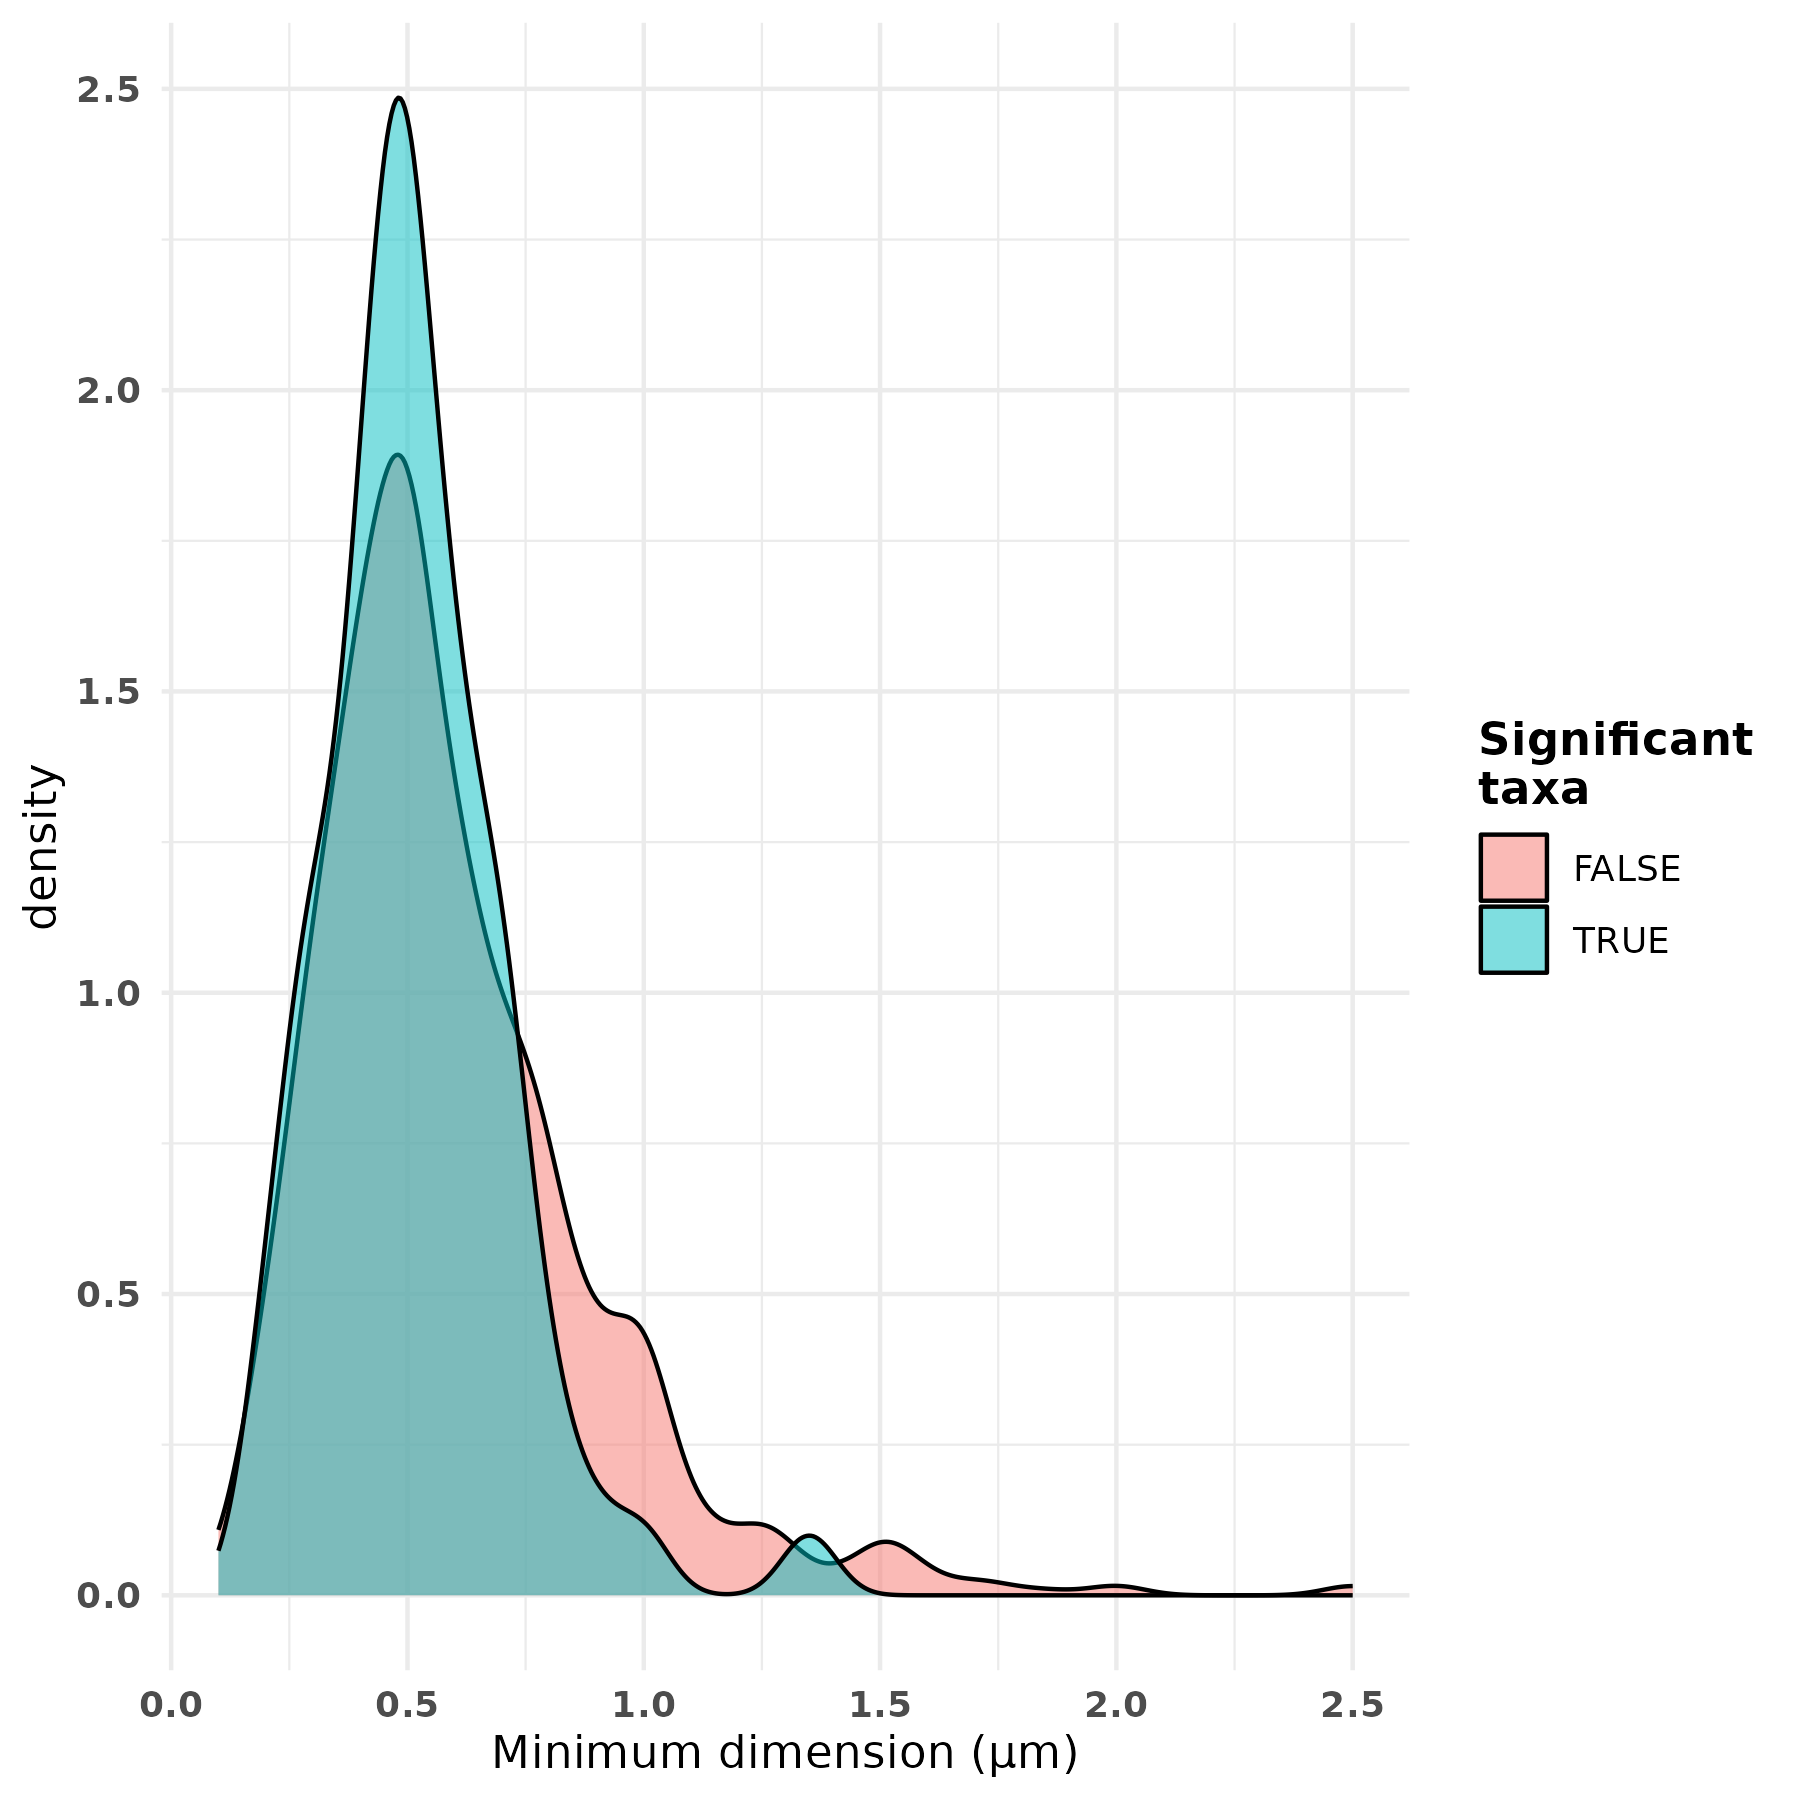
\includegraphics[width=25in]{./figs/minimum_cell_dimension_distribution} \caption{Comparitive distributions of minimum cell dimensions}\label{fig:unnamed-chunk-10}
\end{figure}

GLM model for minimum dimension distribution:

\begin{verbatim}
## min_dimension ~ signifigant_taxa
\end{verbatim}

\begin{table}
\centering
\begin{tabular}{l|r|r|r|r}
\hline
term & estimate & std.error & statistic & p.value\\
\hline
(Intercept) & 0.5995287 & 0.0100756 & 59.502782 & 0.0000000\\
\hline
signifigant\_taxaTRUE & -0.0820287 & 0.0366264 & -2.239603 & 0.0253541\\
\hline
\end{tabular}
\end{table}

\hypertarget{cell-shape}{%
\subsection{Cell shape}\label{cell-shape}}

Chi-square test results for significant taxa cell shapes:

\begin{verbatim}
## 
##  Pearson's Chi-squared test
## 
## data:  .
## X-squared = 7.5206, df = 10, p-value = 0.6755
\end{verbatim}

There is no apparent enrichment in cell shape morphology in significant
taxa

\hypertarget{cell-morphology-data}{%
\subsection{Cell morphology data}\label{cell-morphology-data}}

Data extracted from \href{https://bacdive.dsmz.de/}{BacDive}

\begin{table}
\centering
\begin{tabular}{l|l|l|l|r|r|l|r}
\hline
genus & length & width & shape & min\_length & min\_width & signifigant\_taxa & min\_dimension\\
\hline
Acanthopleuribacter & NA & NA & NA & NA & NA & FALSE & NA\\
\hline
Achromobacter & 1.4-2.8 µm & 0.4-1.1 µm & rod & 1.400 & 0.400 & FALSE & 0.400\\
\hline
Achromobacter & 0.9-1.5 µm & 0.4-0.7 µm & rod & 0.900 & 0.400 & FALSE & 0.400\\
\hline
Achromobacter & 0.9-1.5 µm & 0.4-0.7 µm & rod & 0.900 & 0.400 & FALSE & 0.400\\
\hline
Achromobacter & 0.9-1.5 µm & 0.4-0.7 µm & rod & 0.900 & 0.400 & FALSE & 0.400\\
\hline
Achromobacter & 0.9-2.0 µm & 0.4-0.7 µm & rod & 0.900 & 0.400 & FALSE & 0.400\\
\hline
Achromobacter & 2.5-3.0 µm & 0.8-1.2 µm & coccus & 2.500 & 0.800 & FALSE & 0.800\\
\hline
Acidovorax & 3 µm & 0.45 µm & rod & 3.000 & 0.450 & FALSE & 0.450\\
\hline
Acidovorax & 1.5-2.0 µm & 0.3-0.5 µm & rod & 1.500 & 0.300 & FALSE & 0.300\\
\hline
Acidovorax & 1.8 µm & 0.9 µm & rod & 1.800 & 0.900 & FALSE & 0.900\\
\hline
Acinetobacter & 1.5 µm & 1.5 µm & ovoid & 1.500 & 1.500 & FALSE & 1.500\\
\hline
Acinetobacter & 1.5 µm & 1.5 µm & ovoid & 1.500 & 1.500 & FALSE & 1.500\\
\hline
Actibacter & NA & NA & NA & NA & NA & FALSE & NA\\
\hline
Aequorivita & 4.25 µm & 2 µm & rod & 4.250 & 2.000 & FALSE & 2.000\\
\hline
Aequorivita & 0.5-20 µm & 0.4-0.5 µm & filament & 0.500 & 0.400 & FALSE & 0.400\\
\hline
Aestuariibacter & NA & NA & NA & NA & NA & FALSE & NA\\
\hline
Aestuariispira & NA & NA & NA & NA & NA & FALSE & NA\\
\hline
Afipia & NA & NA & rod & NA & NA & FALSE & NA\\
\hline
Agarivorans & 1.7 µm & 0.8 µm & rod & 1.700 & 0.800 & FALSE & 0.800\\
\hline
Agarivorans & 1.5-1.8 µm & 0.5-0.8 µm & rod & 1.500 & 0.500 & FALSE & 0.500\\
\hline
Ahrensia & 1.5-3.5 µm & 0.6-0.8 µm & rod & 1.500 & 0.600 & FALSE & 0.600\\
\hline
Albidovulum & NA & NA & NA & NA & NA & FALSE & NA\\
\hline
Albimonas & 3 µm & 1 µm & rod & 3.000 & 1.000 & FALSE & 1.000\\
\hline
Alcanivorax & 0.5-1.5 µm & 0.3-0.6 µm & rod & 0.500 & 0.300 & FALSE & 0.300\\
\hline
Alcanivorax & 2.4 µm & 0.5 µm & rod & 2.400 & 0.500 & FALSE & 0.500\\
\hline
Alcanivorax & 1.1 µm & 0.55 µm & rod & 1.100 & 0.550 & FALSE & 0.550\\
\hline
Alcanivorax & 2.05 µm & 0.65 µm & rod & 2.050 & 0.650 & FALSE & 0.650\\
\hline
Alcanivorax & 0.8-2.0 µm & 0.3-0.7 µm & rod & 0.800 & 0.300 & FALSE & 0.300\\
\hline
Algimonas & 2.13 µm & 0.38 µm & rod & 2.130 & 0.380 & FALSE & 0.380\\
\hline
Algimonas & 2.13 µm & 0.37 µm & rod & 2.130 & 0.370 & FALSE & 0.370\\
\hline
Algoriphagus & 0.7-1.9 µm & 0.2-0.5 µm & rod & 0.700 & 0.200 & FALSE & 0.200\\
\hline
Algoriphagus & 1.65 µm & 0.5 µm & rod & 1.650 & 0.500 & FALSE & 0.500\\
\hline
Algoriphagus & 2.8 µm & 0.3 µm & rod & 2.800 & 0.300 & FALSE & 0.300\\
\hline
Algoriphagus & 1.4-2.0 µm & 0.4-0.7 µm & rod & 1.400 & 0.400 & FALSE & 0.400\\
\hline
Algoriphagus & 0.8-1.0 µm & 0.4-0.6 µm & rod & 0.800 & 0.400 & FALSE & 0.400\\
\hline
Algoriphagus & 1.7 µm & 0.65 µm & rod & 1.700 & 0.650 & FALSE & 0.650\\
\hline
Algoriphagus & 2.5 µm & 0.5 µm & rod & 2.500 & 0.500 & FALSE & 0.500\\
\hline
Algoriphagus & 1 µm & 0.3 µm & rod & 1.000 & 0.300 & FALSE & 0.300\\
\hline
Algoriphagus & 1.5-15 µm & 0.5-2.5 µm & rod & 1.500 & 0.500 & FALSE & 0.500\\
\hline
Algoriphagus & 6 µm & 0.6 µm & rod & 6.000 & 0.600 & FALSE & 0.600\\
\hline
Algoriphagus & 6 µm & 0.6 µm & rod & 6.000 & 0.600 & FALSE & 0.600\\
\hline
Algoriphagus & 2.3 µm & 0.35 µm & rod & 2.300 & 0.350 & FALSE & 0.350\\
\hline
Algoriphagus & 6 µm & 0.6 µm & rod & 6.000 & 0.600 & FALSE & 0.600\\
\hline
Algoriphagus & 2.5 µm & 0.5 µm & rod & 2.500 & 0.500 & FALSE & 0.500\\
\hline
Aliiglaciecola & 2 µm & NA & rod & 2.000 & NA & FALSE & NA\\
\hline
Aliiroseovarius & 0.9-6.5 µm & 0.4-0.7 µm & ovoid & 0.900 & 0.400 & FALSE & 0.400\\
\hline
Aliiroseovarius & 2.8 µm & 0.9 µm & rod & 2.800 & 0.900 & FALSE & 0.900\\
\hline
Altererythrobacter & 0.98-1-22 µm & 0.45-0.65 µm & rod & 0.980 & 0.450 & FALSE & 0.450\\
\hline
Altererythrobacter & 0.605 µm & 0.5 µm & rod & 0.605 & 0.500 & FALSE & 0.500\\
\hline
Alteromonas & 1.2-1.7 µm & 0.3-0.6 µm & rod & 1.200 & 0.300 & FALSE & 0.300\\
\hline
Alteromonas & 1.7-1.9 µm & 0.9-1.2 µm & rod & 1.700 & 0.900 & FALSE & 0.900\\
\hline
Alteromonas & 1.5-2.5 µm & 0.3-0.8 µm & rod & 1.500 & 0.300 & FALSE & 0.300\\
\hline
Alteromonas & 0.7-0.8 µm & 0.4-0.8 µm & rod & 0.700 & 0.400 & FALSE & 0.400\\
\hline
Alteromonas & 1.2-2.5 µm & 0.5-0.9 µm & coccus & 1.200 & 0.500 & FALSE & 0.500\\
\hline
Alteromonas & 1.2-2.5 µm & 0.75 µm & rod & 1.200 & 0.750 & FALSE & 0.750\\
\hline
Alteromonas & 1.5 µm & 1 µm & rod & 1.500 & 1.000 & FALSE & 1.000\\
\hline
Alteromonas & 3 µm & 0.7-1.2 µm & rod & 3.000 & 0.700 & FALSE & 0.700\\
\hline
Alteromonas & 1.5-2.2 µm & 0.9 µm & rod & 1.500 & 0.900 & FALSE & 0.900\\
\hline
Alteromonas & 1.8 µm & 0.4 µm & rod & 1.800 & 0.400 & FALSE & 0.400\\
\hline
Amphritea & 0.8-1.5 µm & 0.4-0.6 µm & rod & 0.800 & 0.400 & FALSE & 0.400\\
\hline
Amphritea & 1.3-2 µm & 0.6-0.9 µm & rod & 1.300 & 0.600 & FALSE & 0.600\\
\hline
Amphritea & 0.9-1.7 µm & 0.6-0.9 µm & rod & 0.900 & 0.600 & FALSE & 0.600\\
\hline
Amphritea & 1.25 µm & 0.5 µm & rod & 1.250 & 0.500 & FALSE & 0.500\\
\hline
Anderseniella & 3 µm & 0.75 µm & rod & 3.000 & 0.750 & FALSE & 0.750\\
\hline
Anoxybacillus & 2.5-2.7 µm & 0.8 µm & rod & 2.500 & 0.800 & FALSE & 0.800\\
\hline
Anoxybacillus & 5 µm & 0.9 µm & rod & 5.000 & 0.900 & FALSE & 0.900\\
\hline
Anoxybacillus & 1.4-4 µm & 0.3-0.6 µm & rod & 1.400 & 0.300 & FALSE & 0.300\\
\hline
Anoxybacillus & 3.3 µm & 0.5 µm & rod & 3.300 & 0.500 & FALSE & 0.500\\
\hline
Anoxybacillus & 4.3 µm & 1.05 µm & rod & 4.300 & 1.050 & FALSE & 1.050\\
\hline
Anoxybacillus & 7 µm & 0.85 µm & rod & 7.000 & 0.850 & FALSE & 0.850\\
\hline
Aquabacterium & NA & NA & rod & NA & NA & FALSE & NA\\
\hline
Aquihabitans & NA & NA & NA & NA & NA & FALSE & NA\\
\hline
Aquimarina & 2.5-4.0 µm & 0.4-0.6 µm & rod & 2.500 & 0.400 & FALSE & 0.400\\
\hline
Aquimarina & 3.5-7.0 µm & 0.3-0.5 µm & rod & 3.500 & 0.300 & FALSE & 0.300\\
\hline
Aquimarina & 34.5 µm & 0.3 µm & rod & 34.500 & 0.300 & FALSE & 0.300\\
\hline
Aquimarina & 3-25.5 µm & 0.4-0.6 µm & rod & 3.000 & 0.400 & FALSE & 0.400\\
\hline
Aquimarina & 1.0-2.0 µm & 0.2-0.4 µm & rod & 1.000 & 0.200 & FALSE & 0.200\\
\hline
Aquimarina & 1.8-2 µm & 0.5-0.6 µm & rod & 1.800 & 0.500 & FALSE & 0.500\\
\hline
Arcobacter & 1-2 µm & 0.5-0.8 µm & coccus & 1.000 & 0.500 & FALSE & 0.500\\
\hline
Arcobacter & 0.8-2 µm & 0.4 µm & rod & 0.800 & 0.400 & FALSE & 0.400\\
\hline
Arcobacter & 1.7 µm & 0.2 µm & rod & 1.700 & 0.200 & FALSE & 0.200\\
\hline
Arcobacter & 1.1 µm & 0.5 µm & rod & 1.100 & 0.500 & FALSE & 0.500\\
\hline
Arcobacter & 2.5 µm & 0.5 µm & rod & 2.500 & 0.500 & FALSE & 0.500\\
\hline
Arcobacter & 2 µm & 0.4-0.5 µm & rod & 2.000 & 0.400 & FALSE & 0.400\\
\hline
Arcobacter & 1.5-2.5 µm & 0.5 µm & rod & 1.500 & 0.500 & FALSE & 0.500\\
\hline
Arcobacter & 1.5 µm & 0.2-0.4 µm & rod & 1.500 & 0.200 & FALSE & 0.200\\
\hline
Arcobacter & 1.0-3.0 µm & 0.2-0.4 µm & rod & 1.000 & 0.200 & FALSE & 0.200\\
\hline
Arenicella & 2.7 µm & 0.55 µm & rod & 2.700 & 0.550 & FALSE & 0.550\\
\hline
Arenicella & 3.5 µm & 0.55 µm & rod & 3.500 & 0.550 & FALSE & 0.550\\
\hline
Atopostipes & NA & NA & NA & NA & NA & FALSE & NA\\
\hline
Aureicoccus & 2 µm & 2 µm & coccus & 2.000 & 2.000 & FALSE & 2.000\\
\hline
Aureispira & 4.5 µm & 0.75 µm & rod & 4.500 & 0.750 & FALSE & 0.750\\
\hline
Aureitalea & NA & NA & NA & NA & NA & FALSE & NA\\
\hline
Azonexus & 1.65 µm & 0.4 µm & rod & 1.650 & 0.400 & TRUE & 0.400\\
\hline
Bacteroides & 0.8-5 µm & 0.8-1 µm & rod & 0.800 & 0.800 & FALSE & 0.800\\
\hline
Bacteroides & 0.4-20 µm & 0.4-0.8 µm & rod & 0.400 & 0.400 & FALSE & 0.400\\
\hline
Bacteroides & 2.1 µm & 0.8 µm & rod & 2.100 & 0.800 & FALSE & 0.800\\
\hline
Bacteroides & 8.5 µm & 1.2 µm & rod & 8.500 & 1.200 & FALSE & 1.200\\
\hline
Bacteroides & 2.5 µm & 1.4 µm & rod & 2.500 & 1.400 & FALSE & 1.400\\
\hline
Bacteroides & 1.4-55.0 µm & 1-1.9 µm & rod & 1.400 & 1.000 & FALSE & 1.000\\
\hline
Bacteroides & 1-2.5 µm & 1-1.4 µm & rod & 1.000 & 1.000 & FALSE & 1.000\\
\hline
Bacteroides & 0.7-2.9 µm & 0.5-1 µm & rod & 0.700 & 0.500 & FALSE & 0.500\\
\hline
Bacteroides & 2.85 µm & 0.5 µm & rod & 2.850 & 0.500 & FALSE & 0.500\\
\hline
Bacteroides & 1.7 µm & 0.75 µm & rod & 1.700 & 0.750 & FALSE & 0.750\\
\hline
Bacteroides & 1.9 µm & 1 µm & rod & 1.900 & 1.000 & FALSE & 1.000\\
\hline
Bacteroides & 1.5-4.5 µm & 0.8 µm & rod & 1.500 & 0.800 & FALSE & 0.800\\
\hline
Bacteroides & 01-05 µm & 0.8 µm & rod & 1.000 & 0.800 & FALSE & 0.800\\
\hline
Balneola & 2.6 µm & 0.7 µm & rod & 2.600 & 0.700 & FALSE & 0.700\\
\hline
Balneola & 02-03 µm & 0.2 µm & rod & 2.000 & 0.200 & FALSE & 0.200\\
\hline
Bauldia & NA & NA & NA & NA & NA & FALSE & NA\\
\hline
Bdellovibrio & NA & NA & NA & NA & NA & FALSE & NA\\
\hline
Bizionia & 2 µm & 0.4 µm & rod & 2.000 & 0.400 & FALSE & 0.400\\
\hline
Bizionia & 3.25 µm & 0.45 µm & rod & 3.250 & 0.450 & FALSE & 0.450\\
\hline
Bizionia & 2.5 µm & 0.45 µm & rod & 2.500 & 0.450 & FALSE & 0.450\\
\hline
Bizionia & 2.5 µm & 0.4 µm & rod & 2.500 & 0.400 & FALSE & 0.400\\
\hline
Bizionia & 02-03 µm & 0.2-0.4 µm & rod & 2.000 & 0.200 & FALSE & 0.200\\
\hline
Blastopirellula & 1.1-1.5 µm & 0.6-0.8 µm & other & 1.100 & 0.600 & FALSE & 0.600\\
\hline
Blautia & NA & NA & NA & NA & NA & FALSE & NA\\
\hline
Bradyrhizobium & 2-4 µm & 0.6 µm & rod & 2.000 & 0.600 & TRUE & 0.600\\
\hline
Bradyrhizobium & 2-3 µm & 0.7 µm & rod & 2.000 & 0.700 & TRUE & 0.700\\
\hline
Bradyrhizobium & 1.35 µm & 1.35 µm & rod & 1.350 & 1.350 & TRUE & 1.350\\
\hline
Bradyrhizobium & 1.35 µm & 0.46 µm & rod & 1.350 & 0.460 & TRUE & 0.460\\
\hline
Bradyrhizobium & 2-3 µm & 0.7 µm & rod & 2.000 & 0.700 & TRUE & 0.700\\
\hline
Bradyrhizobium & 1.5-4.5 µm & 0.5 µm & rod & 1.500 & 0.500 & TRUE & 0.500\\
\hline
Bradyrhizobium & 4.5 µm & 0.8 µm & rod & 4.500 & 0.800 & TRUE & 0.800\\
\hline
Brevundimonas & 1-2 µm & 0.3-0.4 µm & rod & 1.000 & 0.300 & FALSE & 0.300\\
\hline
Brevundimonas & 2.75 µm & 0.4 µm & rod & 2.750 & 0.400 & FALSE & 0.400\\
\hline
Brevundimonas & 1.6 µm & 0.5 µm & rod & 1.600 & 0.500 & FALSE & 0.500\\
\hline
Brevundimonas & 5.1-5.6 µm & 1.2-1.8 µm & rod & 5.100 & 1.200 & FALSE & 1.200\\
\hline
Brevundimonas & 1.5-3.5 µm & 0.3-0.7 µm & rod & 1.500 & 0.300 & FALSE & 0.300\\
\hline
Brevundimonas & 2.35 µm & 0.4 µm & rod & 2.350 & 0.400 & FALSE & 0.400\\
\hline
Brevundimonas & 01-03 µm & 0.4-0.6 µm & rod & 1.000 & 0.400 & FALSE & 0.400\\
\hline
Brevundimonas & 2.75 µm & 0.5 µm & rod & 2.750 & 0.500 & FALSE & 0.500\\
\hline
Brumimicrobium & 1.5-2.5 µm & 0.3-0.4 µm & rod & 1.500 & 0.300 & FALSE & 0.300\\
\hline
Brumimicrobium & 0.8-1.5 µm & 0.3-0.4 µm & rod & 0.800 & 0.300 & FALSE & 0.300\\
\hline
Brumimicrobium & 1.25 µm & 0.4 µm & rod & 1.250 & 0.400 & FALSE & 0.400\\
\hline
Burkholderia & 2 µm & NA & rod & 2.000 & NA & FALSE & NA\\
\hline
Caldithrix & 04-12 µm & 0.2-0.3 µm & rod & 4.000 & 0.200 & FALSE & 0.200\\
\hline
Campylobacter & 2.5-5 µm & 0.5-1 µm & rod & 2.500 & 0.500 & FALSE & 0.500\\
\hline
Campylobacter & 1.9-3.3 µm & 0.2-0.4 µm & rod & 1.900 & 0.200 & FALSE & 0.200\\
\hline
Campylobacter & 0.5-1.8 µm & 0.25-0.5 µm & rod & 0.500 & 0.250 & FALSE & 0.250\\
\hline
Campylobacter & 1.2-2.5 µm & 0.2-0.5 µm & rod & 1.200 & 0.200 & FALSE & 0.200\\
\hline
Campylobacter & 2.0-5.0 µm & 0.5-0.8 µm & rod & 2.000 & 0.500 & FALSE & 0.500\\
\hline
Candidatus\_Anammoxoglobus & NA & NA & NA & NA & NA & FALSE & NA\\
\hline
Candidatus\_Brocadia & NA & NA & NA & NA & NA & FALSE & NA\\
\hline
Caulobacter & 1.5-2.1 µm & 0.5-0.6 µm & rod & 1.500 & 0.500 & FALSE & 0.500\\
\hline
Caulobacter & 1.8-3.2 µm & 1.1-1.3 µm & rod & 1.800 & 1.100 & FALSE & 1.100\\
\hline
Caulobacter & 1.55 µm & 0.6 µm & rod & 1.550 & 0.600 & FALSE & 0.600\\
\hline
Celeribacter & 0.8-0.9 µm & 0.4-0.5 µm & rod & 0.800 & 0.400 & FALSE & 0.400\\
\hline
Celeribacter & 0.8 µm & 0.3 µm & rod & 0.800 & 0.300 & FALSE & 0.300\\
\hline
Celeribacter & 0.8-1.8 µm & 0.4-0.9 µm & rod & 0.800 & 0.400 & FALSE & 0.400\\
\hline
Celerinatantimonas & 3 µm & 0.75 µm & rod & 3.000 & 0.750 & FALSE & 0.750\\
\hline
Cerasicoccus & 0.9 µm & 0.9 µm & coccus & 0.900 & 0.900 & FALSE & 0.900\\
\hline
Cesiribacter & 1.5-3.0 µm & 0.4-0.5 µm & rod & 1.500 & 0.400 & FALSE & 0.400\\
\hline
Chromohalobacter & 2.85 µm & 0.4 µm & rod & 2.850 & 0.400 & FALSE & 0.400\\
\hline
Chromohalobacter & 2.3-4.2 µm & 0.35-0.5 µm & rod & 2.300 & 0.350 & FALSE & 0.350\\
\hline
Chromohalobacter & 3.85 µm & 0.65 µm & rod & 3.850 & 0.650 & FALSE & 0.650\\
\hline
Chryseobacterium & 2 µm & 0.65 µm & rod & 2.000 & 0.650 & FALSE & 0.650\\
\hline
Chryseobacterium & 1.5 µm & 0.5 µm & rod & 1.500 & 0.500 & FALSE & 0.500\\
\hline
Chryseobacterium & 2.4 µm & 0.8 µm & rod & 2.400 & 0.800 & FALSE & 0.800\\
\hline
Chryseobacterium & 01-02 µm & 0.4-0.8 µm & rod & 1.000 & 0.400 & FALSE & 0.400\\
\hline
Chryseobacterium & 3 µm & 0.75 µm & rod & 3.000 & 0.750 & FALSE & 0.750\\
\hline
Chryseobacterium & 1.25 µm & 0.5 µm & rod & 1.250 & 0.500 & FALSE & 0.500\\
\hline
Chryseobacterium & 1.2-1.8 µm & 0.6-0.7 µm & rod & 1.200 & 0.600 & FALSE & 0.600\\
\hline
Chryseobacterium & 1.1-2.0 µm & 0.5-0.8 µm & rod & 1.100 & 0.500 & FALSE & 0.500\\
\hline
Chryseobacterium & 1.6-2.0 µm & 0.6-0.8 µm & rod & 1.600 & 0.600 & FALSE & 0.600\\
\hline
Chryseobacterium & 1.2 µm & 0.6 µm & rod & 1.200 & 0.600 & FALSE & 0.600\\
\hline
Chryseobacterium & 1.45 µm & 0.4 µm & rod & 1.450 & 0.400 & FALSE & 0.400\\
\hline
Chryseobacterium & 0.85 µm & 0.39 µm & rod & 0.850 & 0.390 & FALSE & 0.390\\
\hline
Chryseobacterium & 2.75 µm & 0.45 µm & rod & 2.750 & 0.450 & FALSE & 0.450\\
\hline
Chryseobacterium & 2 µm & 1 µm & rod & 2.000 & 1.000 & FALSE & 1.000\\
\hline
Chryseobacterium & 1 µm & 0.5 µm & rod & 1.000 & 0.500 & FALSE & 0.500\\
\hline
Chryseobacterium & 2 µm & 1 µm & rod & 2.000 & 1.000 & FALSE & 1.000\\
\hline
Chryseobacterium & 2 µm & 1 µm & rod & 2.000 & 1.000 & FALSE & 1.000\\
\hline
Chryseobacterium & 1.4-2.7 µm & 0.5-0.6 µm & rod & 1.400 & 0.500 & FALSE & 0.500\\
\hline
Chryseobacterium & 0.9-4 µm & 0.5-1 µm & ovoid & 0.900 & 0.500 & FALSE & 0.500\\
\hline
Chryseobacterium & 1.8 µm & 0.6 µm & rod & 1.800 & 0.600 & FALSE & 0.600\\
\hline
Chryseobacterium & 2.05 µm & 0.55 µm & rod & 2.050 & 0.550 & FALSE & 0.550\\
\hline
Chryseobacterium & 2.55 µm & 1 µm & rod & 2.550 & 1.000 & FALSE & 1.000\\
\hline
Chryseobacterium & 2.25 µm & 0.7 µm & rod & 2.250 & 0.700 & FALSE & 0.700\\
\hline
Chryseobacterium & 1.75 µm & 0.65 µm & rod & 1.750 & 0.650 & FALSE & 0.650\\
\hline
Chryseobacterium & 1.3 µm & 0.8 µm & rod & 1.300 & 0.800 & FALSE & 0.800\\
\hline
Chryseobacterium & 1.3 µm & 0.9 µm & rod & 1.300 & 0.900 & FALSE & 0.900\\
\hline
Chryseobacterium & 3.6 µm & 1.1 µm & rod & 3.600 & 1.100 & FALSE & 1.100\\
\hline
Chryseobacterium & 2 µm & 1.25 µm & rod & 2.000 & 1.250 & FALSE & 1.250\\
\hline
Chryseobacterium & 1 µm & 0.5 µm & rod & 1.000 & 0.500 & FALSE & 0.500\\
\hline
Chryseobacterium & 0.9 µm & 0.5 µm & rod & 0.900 & 0.500 & FALSE & 0.500\\
\hline
Chryseobacterium & 1.7 µm & 0.7 µm & rod & 1.700 & 0.700 & FALSE & 0.700\\
\hline
Chryseobacterium & 1.85 µm & 0.7 µm & rod & 1.850 & 0.700 & FALSE & 0.700\\
\hline
Chryseobacterium & 1.9 µm & 0.75 µm & rod & 1.900 & 0.750 & FALSE & 0.750\\
\hline
Chryseobacterium & 1.2-2 µm & 0.7-1.2 µm & rod & 1.200 & 0.700 & FALSE & 0.700\\
\hline
Chryseobacterium & 2-3.5 µm & 0.7-0.8 µm & rod & 2.000 & 0.700 & FALSE & 0.700\\
\hline
Chryseobacterium & 1.25 µm & 0.65 µm & rod & 1.250 & 0.650 & FALSE & 0.650\\
\hline
Chryseobacterium & 1.65 µm & 0.8 µm & rod & 1.650 & 0.800 & FALSE & 0.800\\
\hline
Chryseobacterium & 1-2.5 µm & 0.6-0.7 µm & rod & 1.000 & 0.600 & FALSE & 0.600\\
\hline
Cloacibacterium & 01-02 µm & 0.2-0.3 µm & rod & 1.000 & 0.200 & FALSE & 0.200\\
\hline
Clostridium\_sensu\_stricto & NA & NA & NA & NA & NA & FALSE & NA\\
\hline
Clostridium\_XlVa & NA & NA & NA & NA & NA & FALSE & NA\\
\hline
Cohaesibacter & 1-6 µm & 0.6-1 µm & rod & 1.000 & 0.600 & FALSE & 0.600\\
\hline
Cohaesibacter & 1.8 µm & 0.45 µm & rod & 1.800 & 0.450 & FALSE & 0.450\\
\hline
Cohaesibacter & 1.9 µm & 0.65 µm & rod & 1.900 & 0.650 & FALSE & 0.650\\
\hline
Cohaesibacter & 2 µm & 0.3 µm & rod & 2.000 & 0.300 & FALSE & 0.300\\
\hline
Comamonas & 2 µm & 1 µm & rod & 2.000 & 1.000 & FALSE & 1.000\\
\hline
Comamonas & 0.6-0.7 µm & 0.3-0.7 µm & coccus & 0.600 & 0.300 & FALSE & 0.300\\
\hline
Comamonas & 1.9-2.1 µm & 0.4-0.7 µm & rod & 1.900 & 0.400 & FALSE & 0.400\\
\hline
Comamonas & 0.9-1.5 µm & 0.35 µm & rod & 0.900 & 0.350 & FALSE & 0.350\\
\hline
Comamonas & 1.35 µm & 0.35 µm & rod & 1.350 & 0.350 & FALSE & 0.350\\
\hline
Comamonas & 1.35 µm & 0.6-0.8 µm & rod & 1.350 & 0.600 & FALSE & 0.600\\
\hline
Comamonas & 0.9-1.5 µm & 0.5 µm & rod & 0.900 & 0.500 & FALSE & 0.500\\
\hline
Comamonas & 1.0-2.0 µm & 0.5-1.0 µm & rod & 1.000 & 0.500 & FALSE & 0.500\\
\hline
Comamonas & 2.0-2.5 µm & 1.0-2.0 µm & rod & 2.000 & 1.000 & FALSE & 1.000\\
\hline
Coraliomargarita & 0.4-0.7 µm & NA & coccus & 0.400 & NA & FALSE & NA\\
\hline
Corallibacter & NA & NA & NA & NA & NA & FALSE & NA\\
\hline
Corallomonas & 1 µm & 0.35 µm & rod & 1.000 & 0.350 & FALSE & 0.350\\
\hline
Croceitalea & 1.4-3.1 µm & 0.4-0.6 µm & rod & 1.400 & 0.400 & FALSE & 0.400\\
\hline
Croceitalea & 1-2.8 µm & 0.3-0.5 µm & rod & 1.000 & 0.300 & FALSE & 0.300\\
\hline
Crocinitomix & 0.9-2.5 µm & 0.2-0.4 µm & rod & 0.900 & 0.200 & FALSE & 0.200\\
\hline
Cryomorpha & NA & NA & NA & NA & NA & FALSE & NA\\
\hline
Curvibacter & NA & NA & NA & NA & NA & FALSE & NA\\
\hline
Dasania & NA & NA & NA & NA & NA & FALSE & NA\\
\hline
Dechloromonas & 1.7 µm & 0.5 µm & rod & 1.700 & 0.500 & FALSE & 0.500\\
\hline
Desulfatibacillum & 1.2-4.5 µm & 0.68 µm & rod & 1.200 & 0.680 & FALSE & 0.680\\
\hline
Desulfatibacillum & 2.0-5.5 µm & 0.6-2.2 µm & rod & 2.000 & 0.600 & FALSE & 0.600\\
\hline
Desulfatitalea & 2.75 µm & 0.55 µm & rod & 2.750 & 0.550 & FALSE & 0.550\\
\hline
Desulfobulbus & 1.6-2.2 µm & 0.9-1.0 µm & oval & 1.600 & 0.900 & FALSE & 0.900\\
\hline
Desulfobulbus & 2.25 µm & 1.25 µm & rod & 2.250 & 1.250 & FALSE & 1.250\\
\hline
Desulfopila & 1.0-2.0 µm & 0.3-0.5 µm & rod & 1.000 & 0.300 & FALSE & 0.300\\
\hline
Desulfopila & 1.9-3.8 µm & 0.7-1.2 µm & rod & 1.900 & 0.700 & FALSE & 0.700\\
\hline
Desulfosarcina & 1.0-1.5 µm & 0.5 µm & rod & 1.000 & 0.500 & FALSE & 0.500\\
\hline
Desulfosarcina & 6.0-27.5 µm & 0.8 µm & rod & 6.000 & 0.800 & FALSE & 0.800\\
\hline
Desulfospira & NA & NA & NA & NA & NA & FALSE & NA\\
\hline
Dokdonia & 2.0-3.2 µm & 0.5 µm & rod & 2.000 & 0.500 & FALSE & 0.500\\
\hline
Dokdonia & 2.5-4 µm & 0.5-0.7 µm & rod & 2.500 & 0.500 & FALSE & 0.500\\
\hline
Dokdonia & 2.5-4 µm & 0.5-0.7 µm & rod & 2.500 & 0.500 & FALSE & 0.500\\
\hline
Dokdonia & 2.5-4 µm & 0.5-0.7 µm & rod & 2.500 & 0.500 & FALSE & 0.500\\
\hline
Draconibacterium & NA & NA & NA & NA & NA & FALSE & NA\\
\hline
Dysgonomonas & NA & NA & NA & NA & NA & FALSE & NA\\
\hline
Ekhidna & NA & NA & rod & NA & NA & FALSE & NA\\
\hline
Elizabethkingia & NA & NA & NA & NA & NA & TRUE & NA\\
\hline
Endozoicomonas & 2-3 µm & 0.5-0.8 µm & rod & 2.000 & 0.500 & FALSE & 0.500\\
\hline
Endozoicomonas & 2 µm & 0.7 µm & rod & 2.000 & 0.700 & FALSE & 0.700\\
\hline
Endozoicomonas & 2 µm & 0.7 µm & rod & 2.000 & 0.700 & FALSE & 0.700\\
\hline
Endozoicomonas & 2 µm & 0.6 µm & rod & 2.000 & 0.600 & FALSE & 0.600\\
\hline
Endozoicomonas & 6.5 µm & 0.6 µm & rod & 6.500 & 0.600 & FALSE & 0.600\\
\hline
Enhydrobacter & NA & NA & NA & NA & NA & FALSE & NA\\
\hline
Enterovibrio & 0.5-1.0 µm & 0.55 µm & rod & 0.500 & 0.550 & FALSE & 0.500\\
\hline
Erythrobacter & 0.8-1.6 µm & 0.2-0.7 µm & rod & 0.800 & 0.200 & FALSE & 0.200\\
\hline
Erythrobacter & 1.3-2.5 µm & 0.6-1.0 µm & rod & 1.300 & 0.600 & FALSE & 0.600\\
\hline
Erythrobacter & 1.0-1.3 µm & 0.2-0.3 µm & rod & 1.000 & 0.200 & FALSE & 0.200\\
\hline
Escherichia/Shigella & NA & NA & NA & NA & NA & FALSE & NA\\
\hline
Euzebyella & 1.2-3.4 µm & 0.3-0.4 µm & rod & 1.200 & 0.300 & FALSE & 0.300\\
\hline
Fabibacter & NA & NA & NA & NA & NA & FALSE & NA\\
\hline
Faecalibacterium & NA & NA & NA & NA & NA & FALSE & NA\\
\hline
Fangia & 1.1 µm & 0.525 µm & rod & 1.100 & 0.525 & FALSE & 0.525\\
\hline
Ferrimonas & 1.5 µm & 0.9 µm & ovoid & 1.500 & 0.900 & FALSE & 0.900\\
\hline
Ferrimonas & 1.35 µm & 0.5 µm & rod & 1.350 & 0.500 & FALSE & 0.500\\
\hline
Ferrimonas & 1.7 µm & 0.35 µm & rod & 1.700 & 0.350 & FALSE & 0.350\\
\hline
Filomicrobium & 1.75 µm & 0.75 µm & rod & 1.750 & 0.750 & FALSE & 0.750\\
\hline
Flavobacterium & 2.5 µm & 0.9 µm & rod & 2.500 & 0.900 & FALSE & 0.900\\
\hline
Flavobacterium & 1.75 µm & 0.35 µm & rod & 1.750 & 0.350 & FALSE & 0.350\\
\hline
Flavobacterium & 2.5 µm & 0.9 µm & rod & 2.500 & 0.900 & FALSE & 0.900\\
\hline
Flavobacterium & 1.25 µm & 0.9 µm & rod & 1.250 & 0.900 & FALSE & 0.900\\
\hline
Flavobacterium & 2.5 µm & 0.8 µm & rod & 2.500 & 0.800 & FALSE & 0.800\\
\hline
Flavobacterium & 5.25 µm & 0.3 µm & rod & 5.250 & 0.300 & FALSE & 0.300\\
\hline
Flavobacterium & 6.75 µm & 1 µm & rod & 6.750 & 1.000 & FALSE & 1.000\\
\hline
Flavobacterium & 4 µm & 1.5 µm & rod & 4.000 & 1.500 & FALSE & 1.500\\
\hline
Flavobacterium & 2 µm & 0.5 µm & rod & 2.000 & 0.500 & FALSE & 0.500\\
\hline
Flavobacterium & 1.5-3 µm & 0.3-0.5 µm & rod & 1.500 & 0.300 & FALSE & 0.300\\
\hline
Flavobacterium & 1.8 µm & 0.5 µm & rod & 1.800 & 0.500 & FALSE & 0.500\\
\hline
Flavobacterium & 5.8-6.3 µm & 0.7-0.8 µm & rod & 5.800 & 0.700 & FALSE & 0.700\\
\hline
Flavobacterium & 2.5 µm & 0.5 µm & rod & 2.500 & 0.500 & FALSE & 0.500\\
\hline
Flavobacterium & 3.5 µm & 0.5 µm & rod & 3.500 & 0.500 & FALSE & 0.500\\
\hline
Flavobacterium & 1.1-2.3 µm & 0.2-0.3 µm & rod & 1.100 & 0.200 & FALSE & 0.200\\
\hline
Flavobacterium & 1.6-12.5 µm & 0.3-0.6 µm & rod & 1.600 & 0.300 & FALSE & 0.300\\
\hline
Flavobacterium & 1.5-2.5 µm & 0.35-0.55 µm & rod & 1.500 & 0.350 & FALSE & 0.350\\
\hline
Flavobacterium & 3-10 µm & 0.3-0.5 µm & rod & 3.000 & 0.300 & FALSE & 0.300\\
\hline
Flavobacterium & 02-03 µm & 0.5 µm & rod & 2.000 & 0.500 & FALSE & 0.500\\
\hline
Flavobacterium & 1.5-2.5 µm & 0.3 µm & rod & 1.500 & 0.300 & FALSE & 0.300\\
\hline
Flavobacterium & 04-06 µm & 1.25 µm & rod & 4.000 & 1.250 & FALSE & 1.250\\
\hline
Flavobacterium & 3.5 µm & 0.5 µm & rod & 3.500 & 0.500 & FALSE & 0.500\\
\hline
Flavobacterium & 2 µm & 0.6 µm & rod & 2.000 & 0.600 & FALSE & 0.600\\
\hline
Flavobacterium & 1.6 µm & 0.4-0.5 µm & rod & 1.600 & 0.400 & FALSE & 0.400\\
\hline
Flavobacterium & 03-04 µm & 0.4-0.5 µm & rod & 3.000 & 0.400 & FALSE & 0.400\\
\hline
Flavobacterium & 03-04 µm & 0.5-0.7 µm & rod & 3.000 & 0.500 & FALSE & 0.500\\
\hline
Flavobacterium & 1-5 µm & 0.3-0.4 µm & rod & 1.000 & 0.300 & FALSE & 0.300\\
\hline
Flavobacterium & 1-5 µm & 0.5-0.7 µm & rod & 1.000 & 0.500 & FALSE & 0.500\\
\hline
Flavobacterium & 2.5-6 µm & 0.4-0.7 µm & rod & 2.500 & 0.400 & FALSE & 0.400\\
\hline
Flexithrix & NA & NA & NA & NA & NA & FALSE & NA\\
\hline
Fluviicola & 1.8-2.5 µm & 0.3-0.6 µm & rod & 1.800 & 0.300 & FALSE & 0.300\\
\hline
Fluviicola & 1.8-2.2 µm & 0.45-0.65 µm & rod & 1.800 & 0.450 & FALSE & 0.450\\
\hline
Fluviicola & 1.6 µm & 0.45 µm & rod & 1.600 & 0.450 & FALSE & 0.450\\
\hline
Francisella & NA & NA & NA & NA & NA & FALSE & NA\\
\hline
Fretibacter & 2.95 µm & 0.45 µm & rod & 2.950 & 0.450 & FALSE & 0.450\\
\hline
Fulvivirga & 5.5 µm & 0.4 µm & rod & 5.500 & 0.400 & FALSE & 0.400\\
\hline
Fusicatenibacter & 8.25 µm & 0.75 µm & rod & 8.250 & 0.750 & FALSE & 0.750\\
\hline
Fusobacterium & NA & NA & NA & NA & NA & FALSE & NA\\
\hline
Gaetbulimicrobium & NA & NA & NA & NA & NA & FALSE & NA\\
\hline
Gangjinia & NA & NA & NA & NA & NA & FALSE & NA\\
\hline
Gemmiger & NA & NA & NA & NA & NA & FALSE & NA\\
\hline
Geobacillus & 3.2-4.5 µm & 0.3-0.8 µm & rod & 3.200 & 0.300 & FALSE & 0.300\\
\hline
Geobacillus & 4.4-5.8 µm & 1.1-1.4 µm & rod & 4.400 & 1.100 & FALSE & 1.100\\
\hline
Geobacillus & 4.7-8.0 µm & 0.9-1.3 µm & rod & 4.700 & 0.900 & FALSE & 0.900\\
\hline
Geobacillus & 4.0-7.0 µm & 0.6-0.8 µm & rod & 4.000 & 0.600 & FALSE & 0.600\\
\hline
Geobacillus & 2.0-6.0 µm & 0.7-1.5 µm & rod & 2.000 & 0.700 & FALSE & 0.700\\
\hline
Geobacillus & 6.0-12.0 µm & 0.9-1.5 µm & rod & 6.000 & 0.900 & FALSE & 0.900\\
\hline
Geobacillus & 2.0-3.5 µm & 0.6-1.0 µm & rod & 2.000 & 0.600 & FALSE & 0.600\\
\hline
Geobacter & 2.75 µm & 0.8 µm & rod & 2.750 & 0.800 & FALSE & 0.800\\
\hline
Gilvibacter & 3.0-5.0 µm & 0.5-0.7 µm & rod & 3.000 & 0.500 & FALSE & 0.500\\
\hline
Gimesia & 1.2-1.8 µm & 0.5-0.9 µm & other & 1.200 & 0.500 & FALSE & 0.500\\
\hline
Gimesia & 1.2-1.4 µm & 0.7-0.9 µm & other & 1.200 & 0.700 & FALSE & 0.700\\
\hline
Gimesia & 1.2-1.6 µm & 0.6-0.8 µm & other & 1.200 & 0.600 & FALSE & 0.600\\
\hline
Gimesia & 1.6-2.2 µm & 1.1-1.5 µm & other & 1.600 & 1.100 & FALSE & 1.100\\
\hline
Gimesia & 1.1-1.5 µm & 0.9-1.1 µm & other & 1.100 & 0.900 & FALSE & 0.900\\
\hline
Glaciecola & NA & NA & NA & NA & NA & FALSE & NA\\
\hline
Gracilimonas & 1.1-1.8 µm & 0.4-0.5 µm & rod & 1.100 & 0.400 & FALSE & 0.400\\
\hline
Gracilimonas & 2.7 µm & 0.3 µm & rod & 2.700 & 0.300 & FALSE & 0.300\\
\hline
Gracilimonas & 7.25 µm & 0.4 µm & rod & 7.250 & 0.400 & FALSE & 0.400\\
\hline
Gracilimonas & 15.35 µm & 0.25 µm & rod & 15.350 & 0.250 & FALSE & 0.250\\
\hline
Granulosicoccus & NA & 1 µm & coccus & NA & 1.000 & FALSE & NA\\
\hline
Grimontia & 1.8-2.8 µm & 0.5-0.7 µm & spiral & 1.800 & 0.500 & FALSE & 0.500\\
\hline
Gynuella & 2.8-3.1 µm & 1.5-1.8 µm & rod & 2.800 & 1.500 & FALSE & 1.500\\
\hline
Haematobacter & NA & NA & NA & NA & NA & FALSE & NA\\
\hline
Haliangium & NA & NA & NA & NA & NA & FALSE & NA\\
\hline
Haliea & 1.6 µm & 0.5 µm & rod & 1.600 & 0.500 & FALSE & 0.500\\
\hline
Haliscomenobacter & NA & NA & NA & NA & NA & FALSE & NA\\
\hline
Halobacteriovorax & 0.5-1 µm & 0.3 µm & vibrio & 0.500 & 0.300 & FALSE & 0.300\\
\hline
Halochromatium & 4 µm & 2.5 µm & rod & 4.000 & 2.500 & FALSE & 2.500\\
\hline
Haloferula & NA & NA & NA & NA & NA & FALSE & NA\\
\hline
Halomonas & 1.6 µm & 1 µm & rod & 1.600 & 1.000 & FALSE & 1.000\\
\hline
Halomonas & 3 µm & 1.3 µm & rod & 3.000 & 1.300 & FALSE & 1.300\\
\hline
Halomonas & 1.5-6 µm & 0.5-0.8 µm & rod & 1.500 & 0.500 & FALSE & 0.500\\
\hline
Halomonas & 2.5 µm & 1 µm & rod & 2.500 & 1.000 & FALSE & 1.000\\
\hline
Halomonas & 2.5 µm & 0.95 µm & rod & 2.500 & 0.950 & FALSE & 0.950\\
\hline
Halomonas & 1.4 µm & 0.5 µm & rod & 1.400 & 0.500 & FALSE & 0.500\\
\hline
Halomonas & 1.85 µm & 0.45 µm & rod & 1.850 & 0.450 & FALSE & 0.450\\
\hline
Halomonas & 2.35 µm & 0.8 µm & rod & 2.350 & 0.800 & FALSE & 0.800\\
\hline
Halomonas & 1.2 µm & 0.7 µm & rod & 1.200 & 0.700 & FALSE & 0.700\\
\hline
Halomonas & 0.8-1.1 µm & 0.5-0.6 µm & rod & 0.800 & 0.500 & FALSE & 0.500\\
\hline
Halomonas & 1.3-1.7 µm & 0.8-1 µm & rod & 1.300 & 0.800 & FALSE & 0.800\\
\hline
Halomonas & 4 µm & 0.75 µm & rod & 4.000 & 0.750 & FALSE & 0.750\\
\hline
Halomonas & 3 µm & 0.75 µm & rod & 3.000 & 0.750 & FALSE & 0.750\\
\hline
Halomonas & 3 µm & 1 µm & coccus & 3.000 & 1.000 & FALSE & 1.000\\
\hline
Halomonas & 3 µm & 1.3 µm & rod & 3.000 & 1.300 & FALSE & 1.300\\
\hline
Halomonas & 1.0-1.6 µm & 0.6-0.8 µm & rod & 1.000 & 0.600 & FALSE & 0.600\\
\hline
Halomonas & 1.2 µm & 0.35 µm & rod & 1.200 & 0.350 & FALSE & 0.350\\
\hline
Halomonas & 1.8-2.4 µm & 0.6-0.8 µm & rod & 1.800 & 0.600 & FALSE & 0.600\\
\hline
Halomonas & 1.6-2 µm & 0.5-0.7 µm & rod & 1.600 & 0.500 & FALSE & 0.500\\
\hline
Halomonas & 1.2-1.6 µm & 0.6-0.8 µm & rod & 1.200 & 0.600 & FALSE & 0.600\\
\hline
Halomonas & 2.25 µm & 0.75 µm & rod & 2.250 & 0.750 & FALSE & 0.750\\
\hline
Halomonas & 2.5 µm & 1.1 µm & rod & 2.500 & 1.100 & FALSE & 1.100\\
\hline
Halomonas & 3.25 µm & 0.86 µm & rod & 3.250 & 0.860 & FALSE & 0.860\\
\hline
Halomonas & 1.3 µm & 0.75 µm & rod & 1.300 & 0.750 & FALSE & 0.750\\
\hline
Halomonas & 2.5 µm & 1.5 µm & rod & 2.500 & 1.500 & FALSE & 1.500\\
\hline
Halomonas & 2.5 µm & 1 µm & rod & 2.500 & 1.000 & FALSE & 1.000\\
\hline
Halomonas & 2.5 µm & 1 µm & rod & 2.500 & 1.000 & FALSE & 1.000\\
\hline
Hanstruepera & NA & NA & NA & NA & NA & FALSE & NA\\
\hline
Hellea & 2.7-5.6 µm & 0.28-0.48 µm & rod & 2.700 & 0.280 & FALSE & 0.280\\
\hline
Hirschia & 2.45 µm & 0.6 µm & coccus & 2.450 & 0.600 & FALSE & 0.600\\
\hline
Hirschia & 1.2-1.3 µm & 0.6-1.1 µm & rod & 1.200 & 0.600 & FALSE & 0.600\\
\hline
Hirschia & 0.5-6 µm & 0.5-1 µm & rod & 0.500 & 0.500 & FALSE & 0.500\\
\hline
Hoeflea & 0.7-2 µm & 0.3-0.5 µm & rod & 0.700 & 0.300 & FALSE & 0.300\\
\hline
Hoeflea & 2.5 µm & 0.8 µm & rod & 2.500 & 0.800 & FALSE & 0.800\\
\hline
Hydrogenophilus & 2.6 µm & 0.4 µm & rod & 2.600 & 0.400 & FALSE & 0.400\\
\hline
Hyphomicrobium & 1.75 µm & 0.65 µm & rod & 1.750 & 0.650 & FALSE & 0.650\\
\hline
Hyphomonas & NA & NA & NA & NA & NA & FALSE & NA\\
\hline
Iamia & 1.45 µm & 0.4 µm & rod & 1.450 & 0.400 & FALSE & 0.400\\
\hline
Idiomarina & 0.8-1.4 µm & 0.2 µm & rod & 0.800 & 0.200 & FALSE & 0.200\\
\hline
Idiomarina & 4.75 µm & 0.45 µm & rod & 4.750 & 0.450 & FALSE & 0.450\\
\hline
Idiomarina & 1.0-2.4 µm & 0.3-0.4 µm & vibrio & 1.000 & 0.300 & FALSE & 0.300\\
\hline
Idiomarina & 2.5 µm & 0.75 µm & rod & 2.500 & 0.750 & FALSE & 0.750\\
\hline
Idiomarina & 3.5 µm & 0.75 µm & rod & 3.500 & 0.750 & FALSE & 0.750\\
\hline
Ignavibacterium & 8.75 µm & 0.25 µm & rod & 8.750 & 0.250 & FALSE & 0.250\\
\hline
Ilumatobacter & 1.4 µm & 0.5 µm & rod & 1.400 & 0.500 & FALSE & 0.500\\
\hline
Ilumatobacter & 0.85 µm & 0.55 µm & rod & 0.850 & 0.550 & FALSE & 0.550\\
\hline
Ilyobacter & NA & NA & NA & NA & NA & FALSE & NA\\
\hline
Jannaschia & 1.0-2.0 µm & 0.6-0.9 µm & rod & 1.000 & 0.600 & FALSE & 0.600\\
\hline
Jannaschia & 1.75 µm & 0.65 µm & rod & 1.750 & 0.650 & FALSE & 0.650\\
\hline
Jannaschia & 1.1-2.3 µm & 0.7-1.2 µm & rod & 1.100 & 0.700 & FALSE & 0.700\\
\hline
Jannaschia & 2.25 µm & 0.6 µm & ovoid & 2.250 & 0.600 & FALSE & 0.600\\
\hline
Jannaschia & 2 µm & 1 µm & rod & 2.000 & 1.000 & FALSE & 1.000\\
\hline
Jannaschia & 1.75 µm & 0.85 µm & rod & 1.750 & 0.850 & FALSE & 0.850\\
\hline
Jannaschia & 1.5 µm & 0.5 µm & rod & 1.500 & 0.500 & FALSE & 0.500\\
\hline
Jannaschia & 1.5 µm & 0.5 µm & rod & 1.500 & 0.500 & FALSE & 0.500\\
\hline
Kangiella & 1.75 µm & 0.75 µm & rod & 1.750 & 0.750 & FALSE & 0.750\\
\hline
Kangiella & 0.95 µm & 0.4 µm & rod & 0.950 & 0.400 & FALSE & 0.400\\
\hline
Kangiella & 2.5-3.5 µm & 0.75 µm & rod & 2.500 & 0.750 & FALSE & 0.750\\
\hline
Kofleria & NA & NA & NA & NA & NA & FALSE & NA\\
\hline
Kordia & 2.45 µm & 0.75 µm & rod & 2.450 & 0.750 & FALSE & 0.750\\
\hline
Kordiimonas & 1.0-2.9 µm & 0.4-0.7 µm & rod & 1.000 & 0.400 & FALSE & 0.400\\
\hline
Kordiimonas & 1.8-3 µm & 0.7-0.9 µm & rod & 1.800 & 0.700 & FALSE & 0.700\\
\hline
Kordiimonas & 3 µm & 0.45 µm & rod & 3.000 & 0.450 & FALSE & 0.450\\
\hline
Kordiimonas & 0.95 µm & 0.75 µm & rod & 0.950 & 0.750 & FALSE & 0.750\\
\hline
Kordiimonas & 4.5 µm & 0.65 µm & rod & 4.500 & 0.650 & FALSE & 0.650\\
\hline
Kordiimonas & 1.35 µm & 0.25 µm & rod & 1.350 & 0.250 & FALSE & 0.250\\
\hline
Lactobacillus & 6.25 µm & 0.5 µm & rod & 6.250 & 0.500 & FALSE & 0.500\\
\hline
Lactobacillus & 20 µm & 0.75 µm & rod & 20.000 & 0.750 & FALSE & 0.750\\
\hline
Lactobacillus & 11 µm & 0.75 µm & rod & 11.000 & 0.750 & FALSE & 0.750\\
\hline
Lactobacillus & 16 µm & 1 µm & rod & 16.000 & 1.000 & FALSE & 1.000\\
\hline
Lactobacillus & 5.75 µm & 1 µm & rod & 5.750 & 1.000 & FALSE & 1.000\\
\hline
Leeuwenhoekiella & 1.4-4.1 µm & 0.4-0.7 µm & rod & 1.400 & 0.400 & FALSE & 0.400\\
\hline
Leeuwenhoekiella & 1.5-4 µm & 0.4-0.7 µm & rod & 1.500 & 0.400 & FALSE & 0.400\\
\hline
Leeuwenhoekiella & 2.3 µm & 0.45 µm & rod & 2.300 & 0.450 & FALSE & 0.450\\
\hline
Legionella & 0.87 µm & 0.61 µm & rod & 0.870 & 0.610 & FALSE & 0.610\\
\hline
Legionella & 1.5 µm & 0.54 µm & rod & 1.500 & 0.540 & FALSE & 0.540\\
\hline
Legionella & 2 µm & 0.66 µm & rod & 2.000 & 0.660 & FALSE & 0.660\\
\hline
Legionella & 1.55 µm & 0.7 µm & rod & 1.550 & 0.700 & FALSE & 0.700\\
\hline
Leisingera & 1.8 µm & 0.9 µm & rod & 1.800 & 0.900 & FALSE & 0.900\\
\hline
Leisingera & 1.4 µm & 1 µm & ovoid & 1.400 & 1.000 & FALSE & 1.000\\
\hline
Lentilitoribacter & NA & NA & NA & NA & NA & FALSE & NA\\
\hline
Lewinella & 2-3.1 µm & 0.6-0.8 µm & rod & 2.000 & 0.600 & FALSE & 0.600\\
\hline
Lewinella & 2-3.2 µm & 0.8-1 µm & rod & 2.000 & 0.800 & FALSE & 0.800\\
\hline
Lewinella & 11.8 µm & 1.15 µm & rod & 11.800 & 1.150 & FALSE & 1.150\\
\hline
Lewinella & 0.8 µm & 0.4 µm & rod & 0.800 & 0.400 & FALSE & 0.400\\
\hline
Lewinella & 0.8 µm & 0.45 µm & rod & 0.800 & 0.450 & FALSE & 0.450\\
\hline
Lewinella & 1.2-2 µm & 0.3-0.5 µm & rod & 1.200 & 0.300 & FALSE & 0.300\\
\hline
Lishizhenia & 2.5 µm & 0.35 µm & rod & 2.500 & 0.350 & FALSE & 0.350\\
\hline
Litoreibacter & 1.3 µm & 0.6 µm & coccus & 1.300 & 0.600 & FALSE & 0.600\\
\hline
Litoreibacter & 1.5 µm & 0.8 µm & ovoid & 1.500 & 0.800 & FALSE & 0.800\\
\hline
Litoreibacter & 1.9 µm & 0.5 µm & rod & 1.900 & 0.500 & FALSE & 0.500\\
\hline
Litoreibacter & 1.9 µm & 0.5 µm & rod & 1.900 & 0.500 & FALSE & 0.500\\
\hline
Litoribrevibacter & 1.5-2.5 µm & 0.4-0.6 µm & rod & 1.500 & 0.400 & FALSE & 0.400\\
\hline
Litorilinea & 100 µm & 0.5 µm & rod & 100.000 & 0.500 & FALSE & 0.500\\
\hline
Litorimonas & 1.5-1.9 µm & 0.6-0.8 µm & rod & 1.500 & 0.600 & FALSE & 0.600\\
\hline
Loktanella & 1.9 µm & 0.8 µm & rod & 1.900 & 0.800 & FALSE & 0.800\\
\hline
Loktanella & 2.5 µm & 0.75 µm & rod & 2.500 & 0.750 & FALSE & 0.750\\
\hline
Loktanella & 3.5 µm & 1 µm & rod & 3.500 & 1.000 & FALSE & 1.000\\
\hline
Luteolibacter & 0.9-1.5 µm & 0.2-0.5 µm & rod & 0.900 & 0.200 & FALSE & 0.200\\
\hline
Luteolibacter & 1.35 µm & 0.65 µm & rod & 1.350 & 0.650 & FALSE & 0.650\\
\hline
Lutibacter & 1-5.7 µm & 0.3-0.8 µm & rod & 1.000 & 0.300 & FALSE & 0.300\\
\hline
Lutibacter & 0.5-10.0 µm & 0.2-0.4 µm & rod & 0.500 & 0.200 & FALSE & 0.200\\
\hline
Lutibacter & 2-6 µm & 0.5 µm & rod & 2.000 & 0.500 & FALSE & 0.500\\
\hline
Lutibacter & 1.2 µm & 0.3 µm & rod & 1.200 & 0.300 & FALSE & 0.300\\
\hline
Lutibacter & 2.6 µm & 0.85 µm & rod & 2.600 & 0.850 & FALSE & 0.850\\
\hline
Lutimaribacter & 2.2-2.5 µm & 0.5-0.8 µm & rod & 2.200 & 0.500 & FALSE & 0.500\\
\hline
Lutimaribacter & 1.1 µm & 0.65 µm & rod & 1.100 & 0.650 & FALSE & 0.650\\
\hline
Lutimonas & 2 µm & 0.85 µm & rod & 2.000 & 0.850 & FALSE & 0.850\\
\hline
Magnetovibrio & 2 µm & 0.3 µm & spiral & 2.000 & 0.300 & FALSE & 0.300\\
\hline
Malonomonas & NA & NA & NA & NA & NA & FALSE & NA\\
\hline
Maricaulis & NA & NA & NA & NA & NA & FALSE & NA\\
\hline
Maricurvus & NA & NA & NA & NA & NA & FALSE & NA\\
\hline
Marinobacter & 1.3-2.2 µm & 0.6-1.2 µm & rod & 1.300 & 0.600 & FALSE & 0.600\\
\hline
Marinobacter & 1.5-2 µm & 0.5-1 µm & rod & 1.500 & 0.500 & FALSE & 0.500\\
\hline
Marinobacter & 2.0-2.5 µm & 0.3-0.5 µm & rod & 2.000 & 0.300 & FALSE & 0.300\\
\hline
Marinobacter & 1.3-2.6 µm & 0.4 µm & rod & 1.300 & 0.400 & FALSE & 0.400\\
\hline
Marinobacter & 1-2.5 µm & 0.5 µm & rod & 1.000 & 0.500 & FALSE & 0.500\\
\hline
Marinobacter & 1.75 µm & 0.35 µm & rod & 1.750 & 0.350 & FALSE & 0.350\\
\hline
Marinobacter & 3 µm & 0.6 µm & rod & 3.000 & 0.600 & FALSE & 0.600\\
\hline
Marinobacter & 2.7 µm & 0.4 µm & rod & 2.700 & 0.400 & FALSE & 0.400\\
\hline
Marinobacter & 1.05 µm & 0.65 µm & ovoid & 1.050 & 0.650 & FALSE & 0.650\\
\hline
Marinobacter & 1-2.5 µm & 0.4-0.8 µm & rod & 1.000 & 0.400 & FALSE & 0.400\\
\hline
Marinobacter & 1.5-3 µm & 0.5-0.8 µm & rod & 1.500 & 0.500 & FALSE & 0.500\\
\hline
Marinobacter & 1.9 µm & 0.65 µm & rod & 1.900 & 0.650 & FALSE & 0.650\\
\hline
Marinobacter & 2.25 µm & 0.7 µm & rod & 2.250 & 0.700 & FALSE & 0.700\\
\hline
Marinobacter & 1.1 µm & 0.45 µm & rod & 1.100 & 0.450 & FALSE & 0.450\\
\hline
Marinobacter & 2.15 µm & 0.75 µm & rod & 2.150 & 0.750 & FALSE & 0.750\\
\hline
Marinobacter & 1.5-2.8 µm & 0.5-0.7 µm & rod & 1.500 & 0.500 & FALSE & 0.500\\
\hline
Marinobacter & 1.7-2.4 µm & 0.6-0.8 µm & rod & 1.700 & 0.600 & FALSE & 0.600\\
\hline
Marinobacter & 1.6-3.0 µm & 0.3-0.5 µm & rod & 1.600 & 0.300 & FALSE & 0.300\\
\hline
Marinobacter & 1.2-4.5 µm & 0.5-1.3 µm & rod & 1.200 & 0.500 & FALSE & 0.500\\
\hline
Marinobacter & 3 µm & 1 µm & rod & 3.000 & 1.000 & FALSE & 1.000\\
\hline
Marinobacter & 1.5 µm & 0.4 µm & rod & 1.500 & 0.400 & FALSE & 0.400\\
\hline
Marinobacter & 6.6 µm & 1.85 µm & rod & 6.600 & 1.850 & FALSE & 1.850\\
\hline
Marinobacter & 1.5-3.0 µm & 0.6-0.8 µm & rod & 1.500 & 0.600 & FALSE & 0.600\\
\hline
Marinobacter & 1.6-2.5 µm & 0.45-0.55 µm & rod & 1.600 & 0.450 & FALSE & 0.450\\
\hline
Marinobacter & 1.5-3.0 µm & 0.6-0.9 µm & rod & 1.500 & 0.600 & FALSE & 0.600\\
\hline
Marinobacter & 1.0-1.3 µm & 0.4-0.5 µm & rod & 1.000 & 0.400 & FALSE & 0.400\\
\hline
Marinobacter & 1.8-2.5 µm & 0.3-0.4 µm & rod & 1.800 & 0.300 & FALSE & 0.300\\
\hline
Marinobacter & 2.5-3.5 µm & 0.3-0.5 µm & rod & 2.500 & 0.300 & FALSE & 0.300\\
\hline
Marinobacter & 2-3 µm & 0.3-0.6 µm & rod & 2.000 & 0.300 & FALSE & 0.300\\
\hline
Marinobacterium & 1.1-1.3 µm & 0.6-0.7 µm & rod & 1.100 & 0.600 & FALSE & 0.600\\
\hline
Marinobacterium & 1.9-2.1 µm & 0.6-0.8 µm & rod & 1.900 & 0.600 & FALSE & 0.600\\
\hline
Marinobacterium & 1.9-2.4 µm & 0.7-1 µm & rod & 1.900 & 0.700 & FALSE & 0.700\\
\hline
Marinobacterium & 0.7-8 µm & 0.4-0.8 µm & rod & 0.700 & 0.400 & FALSE & 0.400\\
\hline
Marinobacterium & 1.0-2.0 µm & 0.4-0.6 µm & rod & 1.000 & 0.400 & FALSE & 0.400\\
\hline
Marinobacterium & 3.5 µm & 1 µm & rod & 3.500 & 1.000 & FALSE & 1.000\\
\hline
Marinobacterium & 0.85 µm & 0.55 µm & rod & 0.850 & 0.550 & FALSE & 0.550\\
\hline
Marinobacterium & 1.5 µm & 0.4 µm & rod & 1.500 & 0.400 & FALSE & 0.400\\
\hline
Marinobacterium & 2 µm & 0.65 µm & rod & 2.000 & 0.650 & FALSE & 0.650\\
\hline
Marinobacterium & 1.3 µm & 0.7 µm & rod & 1.300 & 0.700 & FALSE & 0.700\\
\hline
Marinobacterium & 0.7 µm & 0.35 µm & rod & 0.700 & 0.350 & FALSE & 0.350\\
\hline
Marinobacterium & 1.6-2.3 µm & 0.5-0.7 µm & rod & 1.600 & 0.500 & FALSE & 0.500\\
\hline
Marinomonas & 3.5-4.0 µm & 0.8-1.0 µm & rod & 3.500 & 0.800 & FALSE & 0.800\\
\hline
Marinomonas & 1.0-1.2 µm & 0.2-0.4 µm & rod & 1.000 & 0.200 & FALSE & 0.200\\
\hline
Marinomonas & 1.2-3.9 µm & 0.5-0.9 µm & rod & 1.200 & 0.500 & FALSE & 0.500\\
\hline
Marinomonas & 1.2-2.6 µm & 0.3-0.4 µm & rod & 1.200 & 0.300 & FALSE & 0.300\\
\hline
Marinomonas & 2 µm & 0.5 µm & rod & 2.000 & 0.500 & FALSE & 0.500\\
\hline
Marinomonas & 1.2 µm & 0.6-0.8 µm & rod & 1.200 & 0.600 & FALSE & 0.600\\
\hline
Marinoscillum & 0.35 µm & NA & rod & 0.350 & NA & FALSE & NA\\
\hline
Maritimimonas & NA & NA & NA & NA & NA & FALSE & NA\\
\hline
Marivita & 2.25 µm & 0.6 µm & rod & 2.250 & 0.600 & FALSE & 0.600\\
\hline
Marivita & 2.7 µm & 0.8 µm & rod & 2.700 & 0.800 & FALSE & 0.800\\
\hline
Marixanthomonas & 2.5 µm & 0.45 µm & rod & 2.500 & 0.450 & TRUE & 0.450\\
\hline
Mesoflavibacter & NA & NA & NA & NA & NA & FALSE & NA\\
\hline
Mesonia & 0.8-1.8 µm & 0.5-0.7 µm & rod & 0.800 & 0.500 & FALSE & 0.500\\
\hline
Mesonia & 1-2.1 µm & 0.4-0.5 µm & rod & 1.000 & 0.400 & FALSE & 0.400\\
\hline
Mesonia & 1.6-2.3 µm & 0.4-0.5 µm & rod & 1.600 & 0.400 & FALSE & 0.400\\
\hline
Mesorhizobium & 0.5-1.2 µm & 0.4-0.5 µm & rod & 0.500 & 0.400 & FALSE & 0.400\\
\hline
Mesorhizobium & 0.8-1.5 µm & 0.4-0.5 µm & rod & 0.800 & 0.400 & FALSE & 0.400\\
\hline
Mesorhizobium & 1.4 µm & 0.6 µm & rod & 1.400 & 0.600 & FALSE & 0.600\\
\hline
Mesorhizobium & 0.9-2.0 µm & 0.4-0.6 µm & rod & 0.900 & 0.400 & FALSE & 0.400\\
\hline
Mesorhizobium & 1.13 µm & 0.38 µm & rod & 1.130 & 0.380 & FALSE & 0.380\\
\hline
Mesorhizobium & 2 µm & 1 µm & rod & 2.000 & 1.000 & FALSE & 1.000\\
\hline
Mesorhizobium & 1.5-2.5 µm & 0.6-0.7 µm & rod & 1.500 & 0.600 & FALSE & 0.600\\
\hline
Mesorhizobium & 1.5-3.0 µm & 0.5-0.7 µm & rod & 1.500 & 0.500 & FALSE & 0.500\\
\hline
Mesorhizobium & 1.5-2.0 µm & 1 µm & rod & 1.500 & 1.000 & FALSE & 1.000\\
\hline
Mesorhizobium & 2 µm & 1 µm & rod & 2.000 & 1.000 & FALSE & 1.000\\
\hline
Mesorhizobium & 1.5-3.0 µm & 0.3-0.5 µm & rod & 1.500 & 0.300 & FALSE & 0.300\\
\hline
Mesorhizobium & 02-03 µm & 0.5 µm & rod & 2.000 & 0.500 & FALSE & 0.500\\
\hline
Mesorhizobium & 1 µm & 0.5 µm & rod & 1.000 & 0.500 & FALSE & 0.500\\
\hline
Mesorhizobium & 01-03 µm & 0.3-0.6 µm & rod & 1.000 & 0.300 & FALSE & 0.300\\
\hline
Mesorhizobium & 01-03 µm & 0.3-0.6 µm & rod & 1.000 & 0.300 & FALSE & 0.300\\
\hline
Mesorhizobium & 1.4 µm & 0.6 µm & rod & 1.400 & 0.600 & FALSE & 0.600\\
\hline
Mesorhizobium & 1.5-2.0 µm & 0.3-0.6 µm & rod & 1.500 & 0.300 & FALSE & 0.300\\
\hline
Mesorhizobium & 2.59 µm & 0.34 µm & rod & 2.590 & 0.340 & FALSE & 0.340\\
\hline
Mesorhizobium & 2.61 µm & 0.33 µm & rod & 2.610 & 0.330 & FALSE & 0.330\\
\hline
Mesorhizobium & 2 µm & 0.45 µm & rod & 2.000 & 0.450 & FALSE & 0.450\\
\hline
Mesorhizobium & 1.435 µm & 0.45 µm & rod & 1.435 & 0.450 & FALSE & 0.450\\
\hline
Mesorhizobium & 2.7 µm & 0.3 µm & rod & 2.700 & 0.300 & FALSE & 0.300\\
\hline
Mesorhizobium & 1.65 µm & 0.53 µm & rod & 1.650 & 0.530 & FALSE & 0.530\\
\hline
Mesorhizobium & 3.1 µm & 1.5 µm & rod & 3.100 & 1.500 & FALSE & 1.500\\
\hline
Mesorhizobium & 1-2.5 µm & 0.3-0.6 µm & rod & 1.000 & 0.300 & FALSE & 0.300\\
\hline
Mesorhizobium & 2 µm & 0.45 µm & rod & 2.000 & 0.450 & FALSE & 0.450\\
\hline
Mesorhizobium & 01-03 µm & 0.3-0.5 µm & rod & 1.000 & 0.300 & FALSE & 0.300\\
\hline
Mesorhizobium & 1.2-1.5 µm & 0.2-0.4 µm & rod & 1.200 & 0.200 & FALSE & 0.200\\
\hline
Methylobacterium & 1.25 µm & 0.9 µm & rod & 1.250 & 0.900 & FALSE & 0.900\\
\hline
Methylobacterium & 2.5 µm & 1.1 µm & rod & 2.500 & 1.100 & FALSE & 1.100\\
\hline
Methylobacterium & 2.5 µm & 1.2 µm & rod & 2.500 & 1.200 & FALSE & 1.200\\
\hline
Methylobacterium & 4.1 µm & 1.3 µm & rod & 4.100 & 1.300 & FALSE & 1.300\\
\hline
Methylobacterium & 1.8 µm & 1.3 µm & rod & 1.800 & 1.300 & FALSE & 1.300\\
\hline
Methylobacterium & 1.99 µm & 0.9 µm & rod & 1.990 & 0.900 & FALSE & 0.900\\
\hline
Methylobacterium & 1.6-5.4 µm & 0.8-1.1 µm & rod & 1.600 & 0.800 & FALSE & 0.800\\
\hline
Methylobacterium & 2.9 µm & 1.15 µm & rod & 2.900 & 1.150 & FALSE & 1.150\\
\hline
Methylobacterium & 2.25 µm & 0.64 µm & rod & 2.250 & 0.640 & FALSE & 0.640\\
\hline
Methylobacterium & 3.3 µm & 1.25 µm & ovoid & 3.300 & 1.250 & FALSE & 1.250\\
\hline
Methylobacterium & 3.6 µm & 1.4 µm & ovoid & 3.600 & 1.400 & FALSE & 1.400\\
\hline
Methylobacterium & 3.65 µm & 1.4 µm & ovoid & 3.650 & 1.400 & FALSE & 1.400\\
\hline
Methylobacterium & 3.55 µm & 1.7 µm & rod & 3.550 & 1.700 & FALSE & 1.700\\
\hline
Methylobacterium & 3.4 µm & 1.1 µm & rod & 3.400 & 1.100 & FALSE & 1.100\\
\hline
Methylobacterium & 2 µm & 1 µm & rod & 2.000 & 1.000 & FALSE & 1.000\\
\hline
Methylobacterium & 2.25 µm & 1 µm & rod & 2.250 & 1.000 & FALSE & 1.000\\
\hline
Methylobacterium & 2.425 µm & 0.7 µm & rod & 2.425 & 0.700 & FALSE & 0.700\\
\hline
Methylobacterium & 1.5-5 µm & 1-1.2 µm & rod & 1.500 & 1.000 & FALSE & 1.000\\
\hline
Methylobacterium & 3.5 µm & 1.15 µm & rod & 3.500 & 1.150 & FALSE & 1.150\\
\hline
Methylobacterium & 4 µm & 1.25 µm & rod & 4.000 & 1.250 & FALSE & 1.250\\
\hline
Methylobacterium & 6.25 µm & 1.6 µm & rod & 6.250 & 1.600 & FALSE & 1.600\\
\hline
Methylobacterium & 2.25 µm & 1.25 µm & rod & 2.250 & 1.250 & FALSE & 1.250\\
\hline
Methyloligella & NA & NA & NA & NA & NA & FALSE & NA\\
\hline
Methylophaga & 1 µm & 0.3 µm & rod & 1.000 & 0.300 & FALSE & 0.300\\
\hline
Methylophaga & 1.5 µm & 0.6 µm & rod & 1.500 & 0.600 & FALSE & 0.600\\
\hline
Methylophaga & 1.5 µm & 0.7 µm & rod & 1.500 & 0.700 & FALSE & 0.700\\
\hline
Methylophaga & 1.6 µm & 0.2 µm & rod & 1.600 & 0.200 & FALSE & 0.200\\
\hline
Methylotenera & 0.8-1.2 µm & 0.3-0.7 µm & ovoid & 0.800 & 0.300 & FALSE & 0.300\\
\hline
Microscilla & 10-100 µm & NA & rod & 10.000 & NA & FALSE & NA\\
\hline
Modicisalibacter & 2.5 µm & 0.8 µm & rod & 2.500 & 0.800 & FALSE & 0.800\\
\hline
Mucilaginibacter & 1.7-2.1 µm & 0.4-0.6 µm & rod & 1.700 & 0.400 & TRUE & 0.400\\
\hline
Mucilaginibacter & 0.7-1.5 µm & 0.3-0.6 µm & rod & 0.700 & 0.300 & TRUE & 0.300\\
\hline
Mucilaginibacter & 0.7-1.4 µm & 0.2-0.5 µm & rod & 0.700 & 0.200 & TRUE & 0.200\\
\hline
Mucilaginibacter & 0.6-0.7 µm & 0.4-0.5 µm & rod & 0.600 & 0.400 & TRUE & 0.400\\
\hline
Mucilaginibacter & 1-1.5 µm & 0.2-0.5 µm & rod & 1.000 & 0.200 & TRUE & 0.200\\
\hline
Mucilaginibacter & 2.7-3.2 µm & 0.5-0.8 µm & rod & 2.700 & 0.500 & TRUE & 0.500\\
\hline
Mucilaginibacter & 1.8-3.2 µm & 0.6-0.9 µm & pleomorphic & 1.800 & 0.600 & TRUE & 0.600\\
\hline
Mucilaginibacter & 1.5-2.8 µm & 0.4-0.8 µm & rod & 1.500 & 0.400 & TRUE & 0.400\\
\hline
Mucilaginibacter & 1.9-2.9 µm & 0.82-0.84 µm & rod & 1.900 & 0.820 & TRUE & 0.820\\
\hline
Mucilaginibacter & 0.8-3.5 µm & 0.3-0.7 µm & rod & 0.800 & 0.300 & TRUE & 0.300\\
\hline
Mucilaginibacter & 1.6 µm & 0.46 µm & rod & 1.600 & 0.460 & TRUE & 0.460\\
\hline
Mucilaginibacter & 2.5 µm & 0.5 µm & rod & 2.500 & 0.500 & TRUE & 0.500\\
\hline
Mucilaginibacter & 1.305 µm & 0.385 µm & rod & 1.305 & 0.385 & TRUE & 0.385\\
\hline
Mucilaginibacter & 1.75 µm & 0.5 µm & rod & 1.750 & 0.500 & TRUE & 0.500\\
\hline
Mucilaginibacter & 1.5 µm & 0.6 µm & rod & 1.500 & 0.600 & TRUE & 0.600\\
\hline
Mucilaginibacter & 1.1-1.5 µm & 0.6-0.8 µm & rod & 1.100 & 0.600 & TRUE & 0.600\\
\hline
Mucilaginibacter & 01-04 µm & 0.3-0.5 µm & rod & 1.000 & 0.300 & TRUE & 0.300\\
\hline
Mucilaginibacter & 01-02 µm & 0.4-0.6 µm & rod & 1.000 & 0.400 & TRUE & 0.400\\
\hline
Mucilaginibacter & 01-03 µm & 0.3-0.5 µm & rod & 1.000 & 0.300 & TRUE & 0.300\\
\hline
Mucilaginibacter & 2 µm & 0.6 µm & rod & 2.000 & 0.600 & TRUE & 0.600\\
\hline
Mucilaginibacter & 0.8-1.2 µm & 0.2-0.4 µm & rod & 0.800 & 0.200 & TRUE & 0.200\\
\hline
Mucilaginibacter & 1.1-1.5 µm & 0.3-1.1 µm & rod & 1.100 & 0.300 & TRUE & 0.300\\
\hline
Mucilaginibacter & 1.1-1.3 µm & 0.3-0.4 µm & rod & 1.100 & 0.300 & TRUE & 0.300\\
\hline
Mucilaginibacter & 1.25-2.3 µm & 0.65-0.75 µm & rod & 1.250 & 0.650 & TRUE & 0.650\\
\hline
Mucilaginibacter & 2.15 µm & 0.65 µm & rod & 2.150 & 0.650 & TRUE & 0.650\\
\hline
Mucilaginibacter & 20.75 µm & 0.45 µm & rod & 20.750 & 0.450 & TRUE & 0.450\\
\hline
Muricauda & 1.4-3.3 µm & 0.2-0.3 µm & rod & 1.400 & 0.200 & FALSE & 0.200\\
\hline
Muricauda & 1.7-2.5 µm & 0.4-0.8 µm & rod & 1.700 & 0.400 & FALSE & 0.400\\
\hline
Muricauda & 1.1-3.0 µm & 0.5-0.8 µm & rod & 1.100 & 0.500 & FALSE & 0.500\\
\hline
Muricauda & 0.7-1 µm & 0.3-0.5 µm & rod & 0.700 & 0.300 & FALSE & 0.300\\
\hline
Muricauda & 1.1-5.3 µm & 0.2-0.6 µm & rod & 1.100 & 0.200 & FALSE & 0.200\\
\hline
Muricauda & 1.8-6.0 µm & 0.2-0.4 µm & rod & 1.800 & 0.200 & FALSE & 0.200\\
\hline
Muricauda & 1.7 µm & 0.28 µm & rod & 1.700 & 0.280 & FALSE & 0.280\\
\hline
Muricauda & 5.25 µm & 0.3 µm & rod & 5.250 & 0.300 & FALSE & 0.300\\
\hline
Muricauda & 4.25 µm & 0.35 µm & rod & 4.250 & 0.350 & FALSE & 0.350\\
\hline
Muricauda & 4.25 µm & 0.3 µm & rod & 4.250 & 0.300 & FALSE & 0.300\\
\hline
Muricauda & 11.5 µm & 0.4 µm & rod & 11.500 & 0.400 & FALSE & 0.400\\
\hline
Muricauda & 3 µm & 0.35 µm & rod & 3.000 & 0.350 & FALSE & 0.350\\
\hline
Muricauda & 1.5 µm & 1.5 µm & rod & 1.500 & 1.500 & FALSE & 1.500\\
\hline
Muricauda & 2.7 µm & 0.475 µm & rod & 2.700 & 0.475 & FALSE & 0.475\\
\hline
Muricauda & 2.25 µm & 0.4 µm & rod & 2.250 & 0.400 & FALSE & 0.400\\
\hline
Muricauda & 1.1-2.7 µm & 0.3-0.6 µm & rod & 1.100 & 0.300 & FALSE & 0.300\\
\hline
Namhaeicola & NA & NA & NA & NA & NA & FALSE & NA\\
\hline
Nannocystis & NA & NA & NA & NA & NA & FALSE & NA\\
\hline
Neisseria & 0.5-0.8 µm & 0.4 µm & coccus & 0.500 & 0.400 & FALSE & 0.400\\
\hline
Neisseria & 0.5 µm & 0.5 µm & coccus & 0.500 & 0.500 & FALSE & 0.500\\
\hline
Neisseria & 1.55 µm & 1.55 µm & rod & 1.550 & 1.550 & FALSE & 1.550\\
\hline
Neisseria & 4 µm & 1.25 µm & rod & 4.000 & 1.250 & FALSE & 1.250\\
\hline
Neptuniibacter & 1.9 µm & 0.65 µm & rod & 1.900 & 0.650 & FALSE & 0.650\\
\hline
Neptunomonas & 1.5 µm & 0.75 µm & rod & 1.500 & 0.750 & FALSE & 0.750\\
\hline
Neptunomonas & 1.1 µm & 0.55 µm & rod & 1.100 & 0.550 & FALSE & 0.550\\
\hline
Neptunomonas & 1.6-1.8 µm & 0.6-1 µm & rod & 1.600 & 0.600 & FALSE & 0.600\\
\hline
Neptunomonas & 1.7 µm & 0.9 µm & rod & 1.700 & 0.900 & FALSE & 0.900\\
\hline
Nisaea & 2.5 µm & 0.9 µm & rod & 2.500 & 0.900 & FALSE & 0.900\\
\hline
Nisaea & 2.5 µm & 0.9 µm & rod & 2.500 & 0.900 & FALSE & 0.900\\
\hline
Nitrosomonas & NA & NA & NA & NA & NA & FALSE & NA\\
\hline
Nonlabens & 03-05 µm & 0.5-0.7 µm & rod & 3.000 & 0.500 & FALSE & 0.500\\
\hline
Nonlabens & 2.5 µm & 0.2-0.4 µm & rod & 2.500 & 0.200 & FALSE & 0.200\\
\hline
Nonlabens & 0.5-10.0 µm & 0.5-0.6 µm & rod & 0.500 & 0.500 & FALSE & 0.500\\
\hline
Novosphingobium & 1.0-2.0 µm & 0.1-0.5 µm & rod & 1.000 & 0.100 & FALSE & 0.100\\
\hline
Novosphingobium & 1.0-1.5 µm & 0.3-0.5 µm & rod & 1.000 & 0.300 & FALSE & 0.300\\
\hline
Novosphingobium & 2.0 µm & 1.5 µm & rod & 2.000 & 1.500 & FALSE & 1.500\\
\hline
Novosphingobium & 1 µm & 0.7 µm & rod & 1.000 & 0.700 & FALSE & 0.700\\
\hline
Novosphingobium & 0.8-1.5 µm & 0.5-0.6 µm & rod & 0.800 & 0.500 & FALSE & 0.500\\
\hline
Novosphingobium & 1.0-3.0 µm & 0.5-0.8 µm & rod & 1.000 & 0.500 & FALSE & 0.500\\
\hline
Novosphingobium & 0.8-1 µm & 0.3-0.5 µm & rod & 0.800 & 0.300 & FALSE & 0.300\\
\hline
Novosphingobium & 0.8-2 µm & 0.3-0.5 µm & rod & 0.800 & 0.300 & FALSE & 0.300\\
\hline
Novosphingobium & 1.3-1.9 µm & 0.25-0.55 µm & rod & 1.300 & 0.250 & FALSE & 0.250\\
\hline
Novosphingobium & 1-1.3 µm & 0.2-0.4 µm & rod & 1.000 & 0.200 & FALSE & 0.200\\
\hline
Novosphingobium & 1.0-1.5 µm & 0.5-0.7 µm & rod & 1.000 & 0.500 & FALSE & 0.500\\
\hline
Novosphingobium & 0.8-2.0 µm & 0.5-0.8 µm & rod & 0.800 & 0.500 & FALSE & 0.500\\
\hline
Novosphingobium & 0.9-4.2 µm & 0.6-0.8 µm & rod & 0.900 & 0.600 & FALSE & 0.600\\
\hline
Novosphingobium & 2 µm & 0.8 µm & rod & 2.000 & 0.800 & FALSE & 0.800\\
\hline
Novosphingobium & 2 µm & 0.9 µm & rod & 2.000 & 0.900 & FALSE & 0.900\\
\hline
Novosphingobium & 1.3 µm & 0.7 µm & rod & 1.300 & 0.700 & FALSE & 0.700\\
\hline
Novosphingobium & 1.7 µm & 0.8 µm & rod & 1.700 & 0.800 & FALSE & 0.800\\
\hline
Novosphingobium & 1 µm & 1 µm & rod & 1.000 & 1.000 & FALSE & 1.000\\
\hline
Novosphingobium & 1.6 µm & 0.8 µm & rod & 1.600 & 0.800 & FALSE & 0.800\\
\hline
Novosphingobium & 1.25 µm & 0.65 µm & rod & 1.250 & 0.650 & FALSE & 0.650\\
\hline
Novosphingobium & 1.4 µm & 0.58 µm & rod & 1.400 & 0.580 & FALSE & 0.580\\
\hline
Novosphingobium & 1.5 µm & 0.6 µm & rod & 1.500 & 0.600 & FALSE & 0.600\\
\hline
Novosphingobium & 1.4 µm & 0.8 µm & rod & 1.400 & 0.800 & FALSE & 0.800\\
\hline
Novosphingobium & 2.9 µm & 0.45 µm & rod & 2.900 & 0.450 & FALSE & 0.450\\
\hline
Novosphingobium & 1.05 µm & 0.4 µm & rod & 1.050 & 0.400 & FALSE & 0.400\\
\hline
Novosphingobium & 0.97-1.95 µm & 0.36-0.45 µm & rod & 0.970 & 0.360 & FALSE & 0.360\\
\hline
Oceanibaculum & 1.5-2.5 µm & 0.8-1 µm & rod & 1.500 & 0.800 & FALSE & 0.800\\
\hline
Oceanibaculum & 2.4 µm & 1.05 µm & rod & 2.400 & 1.050 & FALSE & 1.050\\
\hline
Oceanibaculum & 1.9 µm & 0.6 µm & rod & 1.900 & 0.600 & FALSE & 0.600\\
\hline
Oceanicaulis & 1.1 µm & 0.65 µm & rod & 1.100 & 0.650 & FALSE & 0.650\\
\hline
Oceanicola & 1.6 µm & 0.75 µm & rod & 1.600 & 0.750 & FALSE & 0.750\\
\hline
Oceanococcus & NA & NA & NA & NA & NA & FALSE & NA\\
\hline
Oceanospirillum & NA & NA & NA & NA & NA & FALSE & NA\\
\hline
Odoribacter & 9.2 µm & 1.15 µm & rod & 9.200 & 1.150 & FALSE & 1.150\\
\hline
Oleibacter & 2.15 µm & 0.45 µm & rod & 2.150 & 0.450 & FALSE & 0.450\\
\hline
Oleiphilus & NA & NA & NA & NA & NA & FALSE & NA\\
\hline
Olleya & 2.25 µm & 0.4 µm & rod & 2.250 & 0.400 & FALSE & 0.400\\
\hline
Ornithobacterium & NA & NA & NA & NA & NA & FALSE & NA\\
\hline
Owenweeksia & NA & NA & NA & NA & NA & FALSE & NA\\
\hline
Parachlamydia & NA & NA & NA & NA & NA & FALSE & NA\\
\hline
Paracoccus & 0.9-1.2 µm & 0.7-1.1 µm & rod & 0.900 & 0.700 & FALSE & 0.700\\
\hline
Paracoccus & 1.2-1.5 µm & 0.7-0.9 µm & oval & 1.200 & 0.700 & FALSE & 0.700\\
\hline
Paracoccus & 1.2-1.4 µm & 0.8-1.0 µm & rod & 1.200 & 0.800 & FALSE & 0.800\\
\hline
Paracoccus & 0.4-1.5 µm & 0.4-0.7 µm & pleomorphic & 0.400 & 0.400 & FALSE & 0.400\\
\hline
Paracoccus & 0.7-1.7 µm & 0.4-0.6 µm & rod & 0.700 & 0.400 & FALSE & 0.400\\
\hline
Paracoccus & 1.2-1.4 µm & 0.6-0.7 µm & rod & 1.200 & 0.600 & FALSE & 0.600\\
\hline
Paracoccus & 0.9 µm & 0.45 µm & rod & 0.900 & 0.450 & FALSE & 0.450\\
\hline
Paracoccus & 1 µm & 0.65 µm & rod & 1.000 & 0.650 & FALSE & 0.650\\
\hline
Paracoccus & 1.65 µm & 0.5 µm & rod & 1.650 & 0.500 & FALSE & 0.500\\
\hline
Paracoccus & 0.9 µm & 0.45 µm & rod & 0.900 & 0.450 & FALSE & 0.450\\
\hline
Paracoccus & 1 µm & 0.7 µm & rod & 1.000 & 0.700 & FALSE & 0.700\\
\hline
Paracoccus & 1 µm & 1.75 µm & coccus & 1.000 & 1.750 & FALSE & 1.000\\
\hline
Paracoccus & 0.7-2.5 µm & 0.85 µm & rod & 0.700 & 0.850 & FALSE & 0.700\\
\hline
Paracoccus & 1.9 µm & 0.3-0.6 µm & rod & 1.900 & 0.300 & FALSE & 0.300\\
\hline
Paracoccus & 1.75 µm & 0.6 µm & rod & 1.750 & 0.600 & FALSE & 0.600\\
\hline
Paracoccus & 1 µm & 1.15 µm & ovoid & 1.000 & 1.150 & FALSE & 1.000\\
\hline
Paracoccus & 1.1 µm & 1 µm & coccus & 1.100 & 1.000 & FALSE & 1.000\\
\hline
Paracoccus & 4 µm & 0.6 µm & rod & 4.000 & 0.600 & FALSE & 0.600\\
\hline
Parvibaculum & 1.2-1.4 µm & 0.5-0.6 µm & rod & 1.200 & 0.500 & FALSE & 0.500\\
\hline
Parvibaculum & 1.4 µm & 0.4 µm & rod & 1.400 & 0.400 & FALSE & 0.400\\
\hline
Parvibaculum & 1.4 µm & 0.45 µm & rod & 1.400 & 0.450 & FALSE & 0.450\\
\hline
Parvularcula & 0.6-2.0 µm & 0.3-0.8 µm & rod & 0.600 & 0.300 & FALSE & 0.300\\
\hline
Parvularcula & 2 µm & 0.55 µm & rod & 2.000 & 0.550 & FALSE & 0.550\\
\hline
Parvularcula & 1.45 µm & 0.85 µm & rod & 1.450 & 0.850 & FALSE & 0.850\\
\hline
Pelagibacterium & 1.0-1.5 µm & 0.4-0.8 µm & rod & 1.000 & 0.400 & FALSE & 0.400\\
\hline
Pelagibacterium & 0.8-1.3 µm & 0.3-0.6 µm & rod & 0.800 & 0.300 & FALSE & 0.300\\
\hline
Pelagibacterium & 0.7-1.1 µm & 0.6-0.7 µm & rod & 0.700 & 0.600 & FALSE & 0.600\\
\hline
Pelagibacterium & 1.2-2.5 µm & 0.5-0.6 µm & rod & 1.200 & 0.500 & FALSE & 0.500\\
\hline
Pelagibius & 1.85 µm & 0.75 µm & rod & 1.850 & 0.750 & FALSE & 0.750\\
\hline
Pelagicoccus & NA & NA & NA & NA & NA & FALSE & NA\\
\hline
Peredibacter & NA & NA & NA & NA & NA & FALSE & NA\\
\hline
Perspicuibacter & NA & NA & NA & NA & NA & FALSE & NA\\
\hline
Phaeocystidibacter & 1.25 µm & 0.3 µm & rod & 1.250 & 0.300 & FALSE & 0.300\\
\hline
Phaeodactylibacter & NA & NA & NA & NA & NA & FALSE & NA\\
\hline
Phenylobacterium & 1.2-1.6 µm & 0.5-0.6 µm & rod & 1.200 & 0.500 & FALSE & 0.500\\
\hline
Phenylobacterium & 0.8-1 µm & 0.2-0.3 µm & rod & 0.800 & 0.200 & FALSE & 0.200\\
\hline
Phenylobacterium & 1.4-2.9 µm & 0.6-1.7 µm & rod & 1.400 & 0.600 & FALSE & 0.600\\
\hline
Phenylobacterium & 0.4-1.3 µm & 0.4-0.5 µm & rod & 0.400 & 0.400 & FALSE & 0.400\\
\hline
Phenylobacterium & 2.5-4.0 µm & 0.4-0.6 µm & rod & 2.500 & 0.400 & FALSE & 0.400\\
\hline
Phenylobacterium & 0.7-1.3 µm & 0.5-0.6 µm & ovoid & 0.700 & 0.500 & FALSE & 0.500\\
\hline
Phenylobacterium & 0.8-1.8 µm & 0.5 µm & rod & 0.800 & 0.500 & FALSE & 0.500\\
\hline
Phenylobacterium & 2 µm & 0.5 µm & rod & 2.000 & 0.500 & FALSE & 0.500\\
\hline
Phycisphaera & NA & NA & NA & NA & NA & FALSE & NA\\
\hline
Phyllobacterium & 0.9-3.5 µm & 0.5-0.9 µm & rod & 0.900 & 0.500 & FALSE & 0.500\\
\hline
Phyllobacterium & 1.15 µm & 0.55 µm & rod & 1.150 & 0.550 & FALSE & 0.550\\
\hline
Pibocella & NA & NA & NA & NA & NA & FALSE & NA\\
\hline
Pirellula & NA & NA & NA & NA & NA & FALSE & NA\\
\hline
Planctomicrobium & NA & NA & NA & NA & NA & FALSE & NA\\
\hline
Plesiocystis & NA & NA & NA & NA & NA & FALSE & NA\\
\hline
Polaribacter & 1.1-1.6 µm & 0.4-0.5 µm & rod & 1.100 & 0.400 & FALSE & 0.400\\
\hline
Polaribacter & 1.39 µm & 0.37 µm & rod & 1.390 & 0.370 & FALSE & 0.370\\
\hline
Polaribacter & 1.7-2.0 µm & 0.6-1.0 µm & rod & 1.700 & 0.600 & FALSE & 0.600\\
\hline
Polaribacter & 0.8-5 µm & 0.4-0.6 µm & rod & 0.800 & 0.400 & FALSE & 0.400\\
\hline
Ponticaulis & NA & NA & NA & NA & NA & FALSE & NA\\
\hline
Portibacter & NA & NA & NA & NA & NA & FALSE & NA\\
\hline
Prevotella & 3 µm & 0.8 µm & rod & 3.000 & 0.800 & FALSE & 0.800\\
\hline
Prevotella & 1.6 µm & 0.65 µm & rod & 1.600 & 0.650 & FALSE & 0.650\\
\hline
Prevotella & 0.8-3 µm & 0.7 µm & rod & 0.800 & 0.700 & FALSE & 0.700\\
\hline
Prevotella & 1.7 µm & 0.75 µm & rod & 1.700 & 0.750 & FALSE & 0.750\\
\hline
Prevotella & 2 µm & 0.7 µm & rod & 2.000 & 0.700 & FALSE & 0.700\\
\hline
Prevotella & 1.1 µm & 0.4 µm & rod & 1.100 & 0.400 & FALSE & 0.400\\
\hline
Prevotella & 0.75 µm & 0.45 µm & rod & 0.750 & 0.450 & FALSE & 0.450\\
\hline
Prevotella & 1.16 µm & 0.33 µm & rod & 1.160 & 0.330 & FALSE & 0.330\\
\hline
Prevotella & 0.95 µm & 0.83 µm & rod & 0.950 & 0.830 & FALSE & 0.830\\
\hline
Prevotella & 0.8-6 µm & 0.7-0.8 µm & rod & 0.800 & 0.700 & FALSE & 0.700\\
\hline
Prevotella & 5.4 µm & 0.8 µm & coccus & 5.400 & 0.800 & FALSE & 0.800\\
\hline
Prevotella & 1.95 µm & 0.4 µm & rod & 1.950 & 0.400 & FALSE & 0.400\\
\hline
Prevotella & 1.3 µm & 0.6 µm & ovoid & 1.300 & 0.600 & FALSE & 0.600\\
\hline
Prevotella & 9.15 µm & 0.65 µm & rod & 9.150 & 0.650 & FALSE & 0.650\\
\hline
Prevotella & 1.25 µm & 0.65 µm & rod & 1.250 & 0.650 & FALSE & 0.650\\
\hline
Propionigenium & NA & NA & NA & NA & NA & FALSE & NA\\
\hline
Propionivibrio & NA & NA & NA & NA & NA & FALSE & NA\\
\hline
Pseudoalteromonas & 0.5-3.5 µm & 0.2-0.7 µm & rod & 0.500 & 0.200 & FALSE & 0.200\\
\hline
Pseudoalteromonas & 1.8-3 µm & 0.8-1.3 µm & rod & 1.800 & 0.800 & FALSE & 0.800\\
\hline
Pseudoalteromonas & 1.4-2.6 µm & 0.5-0.8 µm & rod & 1.400 & 0.500 & FALSE & 0.500\\
\hline
Pseudoalteromonas & 1.3-4.0 µm & 0.4-1.3 µm & rod & 1.300 & 0.400 & FALSE & 0.400\\
\hline
Pseudoalteromonas & 1.35 µm & 0.5 µm & rod & 1.350 & 0.500 & FALSE & 0.500\\
\hline
Pseudoalteromonas & 1.25 µm & 0.65 µm & rod & 1.250 & 0.650 & FALSE & 0.650\\
\hline
Pseudoalteromonas & 1.1-2.8 µm & 0.4-0.7 µm & rod & 1.100 & 0.400 & FALSE & 0.400\\
\hline
Pseudoalteromonas & 1.5-2.2 µm & 0.4-0.5 µm & rod & 1.500 & 0.400 & FALSE & 0.400\\
\hline
Pseudoalteromonas & 01-02 µm & 0.5-0.8 µm & rod & 1.000 & 0.500 & FALSE & 0.500\\
\hline
Pseudoalteromonas & 0.4-0.7 µm & 0.7-0.9 µm & rod & 0.400 & 0.700 & FALSE & 0.400\\
\hline
Pseudoalteromonas & 1.5-3.0 µm & 0.5-0.8 µm & rod & 1.500 & 0.500 & FALSE & 0.500\\
\hline
Pseudobacteriovorax & NA & NA & NA & NA & NA & FALSE & NA\\
\hline
Pseudofulvibacter & 1.8-2.3 µm & 0.4-0.6 µm & rod & 1.800 & 0.400 & FALSE & 0.400\\
\hline
Pseudofulvibacter & 1.2-2 µm & 0.3 µm & rod & 1.200 & 0.300 & FALSE & 0.300\\
\hline
Pseudofulvibacter & 2.9 µm & 0.45 µm & rod & 2.900 & 0.450 & FALSE & 0.450\\
\hline
Pseudohongiella & 1.3-1.7 µm & 0.5-0.7 µm & rod & 1.300 & 0.500 & FALSE & 0.500\\
\hline
Pseudomonas & NA & NA & NA & NA & NA & FALSE & NA\\
\hline
Pseudoruegeria & 0.4-10.0 µm & 0.4-0.8 µm & rod & 0.400 & 0.400 & FALSE & 0.400\\
\hline
Pseudoruegeria & 2.4-2.5 µm & 0.5-0.6 µm & rod & 2.400 & 0.500 & FALSE & 0.500\\
\hline
Pseudoruegeria & 2.8 µm & 0.65 µm & rod & 2.800 & 0.650 & FALSE & 0.650\\
\hline
Pseudoteredinibacter & NA & NA & NA & NA & NA & FALSE & NA\\
\hline
Pseudozobellia & NA & NA & NA & NA & NA & FALSE & NA\\
\hline
Psychrobacter & 0.7-1.3 µm & 0.5-0.8 µm & coccus & 0.700 & 0.500 & FALSE & 0.500\\
\hline
Psychrobacter & 1.15 µm & 0.65 µm & coccus & 1.150 & 0.650 & FALSE & 0.650\\
\hline
Psychrobacter & 1.45 µm & 1 µm & coccus & 1.450 & 1.000 & FALSE & 1.000\\
\hline
Psychrobacter & 1.75 µm & 0.8 µm & ovoid & 1.750 & 0.800 & FALSE & 0.800\\
\hline
Psychrobacter & 1.6-1.9 µm & 0.9-1.1 µm & ovoid & 1.600 & 0.900 & FALSE & 0.900\\
\hline
Psychrobacter & 1.0-2.0 µm & 0.5-1.0 µm & ovoid & 1.000 & 0.500 & FALSE & 0.500\\
\hline
Psychrobacter & 1.62 µm & 0.73 µm & rod & 1.620 & 0.730 & FALSE & 0.730\\
\hline
Psychrobacter & 0.9-1.3 µm & 0.5-0.8 µm & ovoid & 0.900 & 0.500 & FALSE & 0.500\\
\hline
Psychrobacter & 1.55 µm & 1.25 µm & ovoid & 1.550 & 1.250 & FALSE & 1.250\\
\hline
Psychrobium & NA & NA & NA & NA & NA & FALSE & NA\\
\hline
Psychroflexus & 0.6-2.0 µm & 0.2-0.5 µm & rod & 0.600 & 0.200 & FALSE & 0.200\\
\hline
Psychroflexus & 1.2-2.2 µm & 0.3-0.6 µm & rod & 1.200 & 0.300 & FALSE & 0.300\\
\hline
Psychroflexus & 0.3-10.0 µm & 0.2-0.5 µm & rod & 0.300 & 0.200 & FALSE & 0.200\\
\hline
Psychroflexus & 3.0-6.0 µm & 0.4-1.0 µm & rod & 3.000 & 0.400 & FALSE & 0.400\\
\hline
Psychroflexus & 3 µm & 0.55 µm & rod & 3.000 & 0.550 & FALSE & 0.550\\
\hline
Psychroflexus & 2.25 µm & 0.21 µm & rod & 2.250 & 0.210 & FALSE & 0.210\\
\hline
Psychrosphaera & NA & NA & rod & NA & NA & FALSE & NA\\
\hline
Ralstonia & 1.5-3.0 µm & 1.0 µm & rod & 1.500 & 1.000 & FALSE & 1.000\\
\hline
Reichenbachiella & NA & NA & NA & NA & NA & FALSE & NA\\
\hline
Reinekea & 2.1-3.1 µm & 0.15-0.3 µm & rod & 2.100 & 0.150 & FALSE & 0.150\\
\hline
Reinekea & 2.0-4.0 µm & 0.2-0.4 µm & rod & 2.000 & 0.200 & FALSE & 0.200\\
\hline
Reinekea & 2 µm & 0.5 µm & rod & 2.000 & 0.500 & FALSE & 0.500\\
\hline
Reinekea & 1.6 µm & 0.45 µm & rod & 1.600 & 0.450 & FALSE & 0.450\\
\hline
Rhizobium & 1.58 µm & 0.5 µm & rod & 1.580 & 0.500 & TRUE & 0.500\\
\hline
Rhizobium & 3.5 µm & 0.9 µm & rod & 3.500 & 0.900 & TRUE & 0.900\\
\hline
Rhizobium & 2.4 µm & 1 µm & rod & 2.400 & 1.000 & TRUE & 1.000\\
\hline
Rhizobium & 2 µm & 0.55 µm & rod & 2.000 & 0.550 & TRUE & 0.550\\
\hline
Rhizobium & 01-03 µm & 0.3-0.5 µm & rod & 1.000 & 0.300 & TRUE & 0.300\\
\hline
Rhizobium & 2-2.5 µm & 0.5-0.7 µm & rod & 2.000 & 0.500 & TRUE & 0.500\\
\hline
Rhizobium & 1.2 µm & 0.65 µm & rod & 1.200 & 0.650 & TRUE & 0.650\\
\hline
Rhodopirellula & 1.7-2.3 µm & 1.1-1.5 µm & other & 1.700 & 1.100 & FALSE & 1.100\\
\hline
Rhodopirellula & 1.9-2.7 µm & 0.8-1.2 µm & other & 1.900 & 0.800 & FALSE & 0.800\\
\hline
Rhodopirellula & 2.1-2.7 µm & 1.7-2.1 µm & pleomorphic & 2.100 & 1.700 & FALSE & 1.700\\
\hline
Rhodopirellula & 1.75 µm & 1.75 µm & ovoid & 1.750 & 1.750 & FALSE & 1.750\\
\hline
Rhodopseudomonas & 2-4.5 µm & 0.8-1.5 µm & rod & 2.000 & 0.800 & FALSE & 0.800\\
\hline
Rhodopseudomonas & 2.75 µm & 0.9 µm & rod & 2.750 & 0.900 & FALSE & 0.900\\
\hline
Rhodopseudomonas & 4 µm & 0.9 µm & rod & 4.000 & 0.900 & FALSE & 0.900\\
\hline
Rhodospirillum & NA & NA & NA & NA & NA & TRUE & NA\\
\hline
Rhodovibrio & NA & NA & NA & NA & NA & FALSE & NA\\
\hline
Rhodovulum & 1.75 µm & 0.6 µm & rod & 1.750 & 0.600 & FALSE & 0.600\\
\hline
Rhodovulum & 1.75 µm & 0.55 µm & rod & 1.750 & 0.550 & FALSE & 0.550\\
\hline
Rhodovulum & 1.5-1.8 µm & 0.5-1 µm & rod & 1.500 & 0.500 & FALSE & 0.500\\
\hline
Rhodovulum & 1.2 µm & 0.9 µm & rod & 1.200 & 0.900 & FALSE & 0.900\\
\hline
Rhodovulum & 1 µm & 0.5 µm & rod & 1.000 & 0.500 & FALSE & 0.500\\
\hline
Rhodovulum & 01-02 µm & 0.6-0.8 µm & ovoid & 1.000 & 0.600 & FALSE & 0.600\\
\hline
Rickettsia & 1.5 µm & 0.3 µm & rod & 1.500 & 0.300 & FALSE & 0.300\\
\hline
Rickettsia & 1.4 µm & 0.4 µm & rod & 1.400 & 0.400 & FALSE & 0.400\\
\hline
Rickettsia & 0.6-2 µm & 0.4 µm & rod & 0.600 & 0.400 & FALSE & 0.400\\
\hline
Rickettsia & 0.832 µm & 0.427 µm & rod & 0.832 & 0.427 & FALSE & 0.427\\
\hline
Rivicola & NA & NA & NA & NA & NA & FALSE & NA\\
\hline
Robiginitalea & NA & NA & NA & NA & NA & FALSE & NA\\
\hline
Romboutsia & NA & NA & NA & NA & NA & FALSE & NA\\
\hline
Roseburia & NA & NA & NA & NA & NA & FALSE & NA\\
\hline
Roseibacillus & NA & NA & NA & NA & NA & FALSE & NA\\
\hline
Roseibium & 2.0-4.0 µm & 0.5-0.8 µm & rod & 2.000 & 0.500 & FALSE & 0.500\\
\hline
Roseibium & 1.0-2.5 µm & 0.5-1.0 µm & rod & 1.000 & 0.500 & FALSE & 0.500\\
\hline
Roseibium & 1.95 µm & 0.6 µm & rod & 1.950 & 0.600 & FALSE & 0.600\\
\hline
Roseicyclus & 1-2.5 µm & 0.4-0.8 µm & rod & 1.000 & 0.400 & FALSE & 0.400\\
\hline
Roseivirga & 2.0-9.0 µm & 0.4-1.0 µm & rod & 2.000 & 0.400 & FALSE & 0.400\\
\hline
Roseivirga & 1-2 µm & 0.5-0.8 µm & rod & 1.000 & 0.500 & FALSE & 0.500\\
\hline
Roseivirga & 2 µm & 0.5 µm & rod & 2.000 & 0.500 & FALSE & 0.500\\
\hline
Roseivirga & 1.5 µm & 0.5 µm & rod & 1.500 & 0.500 & FALSE & 0.500\\
\hline
Roseivirga & 2.65 µm & 0.4 µm & rod & 2.650 & 0.400 & FALSE & 0.400\\
\hline
Roseivirga & 3.25 µm & 0.6 µm & rod & 3.250 & 0.600 & FALSE & 0.600\\
\hline
Roseivivax & 1.5 µm & 0.85 µm & rod & 1.500 & 0.850 & FALSE & 0.850\\
\hline
Roseovarius & 0.9-2.6 µm & 0.3-1.0 µm & rod & 0.900 & 0.300 & FALSE & 0.300\\
\hline
Roseovarius & 8.1-10.9 µm & 2.5-3.4 µm & rod & 8.100 & 2.500 & FALSE & 2.500\\
\hline
Roseovarius & 2-5.5 µm & 0.3-0.4 µm & rod & 2.000 & 0.300 & FALSE & 0.300\\
\hline
Roseovarius & 1.2-1.8 µm & 0.7-0.9 µm & rod & 1.200 & 0.700 & FALSE & 0.700\\
\hline
Roseovarius & 1.42-3.37 µm & 0.58-0.84 µm & ovoid & 1.420 & 0.580 & FALSE & 0.580\\
\hline
Roseovarius & 1.34 µm & 0.53 µm & rod & 1.340 & 0.530 & FALSE & 0.530\\
\hline
Roseovarius & 2.5 µm & 0.6 µm & ovoid & 2.500 & 0.600 & FALSE & 0.600\\
\hline
Roseovarius & 2.15 µm & 0.6 µm & rod & 2.150 & 0.600 & FALSE & 0.600\\
\hline
Rubinisphaera & 1.4-1.8 µm & 0.7-0.9 µm & other & 1.400 & 0.700 & FALSE & 0.700\\
\hline
Rubricoccus & NA & NA & NA & NA & NA & FALSE & NA\\
\hline
Rubritalea & 1.1-1.4 µm & 0.9-1 µm & rod & 1.100 & 0.900 & FALSE & 0.900\\
\hline
Ruegeria & 1-3 µm & 0.5-1 µm & rod & 1.000 & 0.500 & FALSE & 0.500\\
\hline
Ruegeria & 2.0-5.0 µm & 0.6-1.2 µm & rod & 2.000 & 0.600 & FALSE & 0.600\\
\hline
Ruegeria & 3.5 µm & 1.1 µm & coccus & 3.500 & 1.100 & FALSE & 1.100\\
\hline
Ruegeria & 0.75 µm & 0.4 µm & rod & 0.750 & 0.400 & FALSE & 0.400\\
\hline
Ruegeria & 3.25 µm & 0.75 µm & rod & 3.250 & 0.750 & FALSE & 0.750\\
\hline
Ruminococcus & NA & 0.9-1.3 µm & coccus & NA & 0.900 & FALSE & NA\\
\hline
Ruminococcus2 & NA & NA & NA & NA & NA & FALSE & NA\\
\hline
Saccharicrinis & NA & NA & NA & NA & NA & FALSE & NA\\
\hline
Saccharophagus & NA & NA & NA & NA & NA & FALSE & NA\\
\hline
Salinibacter & NA & NA & NA & NA & NA & FALSE & NA\\
\hline
Salinirepens & 18 µm & 0.55 µm & rod & 18.000 & 0.550 & FALSE & 0.550\\
\hline
Salinisphaera & 1.2-1.6 µm & 0.6-0.7 µm & rod & 1.200 & 0.600 & FALSE & 0.600\\
\hline
Salinisphaera & 1.4 µm & 1 µm & rod & 1.400 & 1.000 & FALSE & 1.000\\
\hline
Salinisphaera & 1.75 µm & 0.6 µm & rod & 1.750 & 0.600 & FALSE & 0.600\\
\hline
Salinisphaera & 1.15 µm & 0.5 µm & rod & 1.150 & 0.500 & FALSE & 0.500\\
\hline
Salinisphaera & 0.9 µm & 0.4 µm & rod & 0.900 & 0.400 & FALSE & 0.400\\
\hline
Salinisphaera & 0.7 µm & 0.45 µm & rod & 0.700 & 0.450 & FALSE & 0.450\\
\hline
Salinispira & NA & NA & NA & NA & NA & FALSE & NA\\
\hline
Salisaeta & 22.5 µm & NA & rod & 22.500 & NA & FALSE & NA\\
\hline
Sandaracinus & 4.5 µm & 0.85 µm & rod & 4.500 & 0.850 & FALSE & 0.850\\
\hline
Saprospira & NA & NA & NA & NA & NA & FALSE & NA\\
\hline
Sebaldella & NA & NA & NA & NA & NA & FALSE & NA\\
\hline
Sediminibacter & 1.0-2.5 µm & 0.5-0.7 µm & rod & 1.000 & 0.500 & FALSE & 0.500\\
\hline
Seonamhaeicola & 1-4 µm & 0.3-0.8 µm & rod & 1.000 & 0.300 & FALSE & 0.300\\
\hline
Seonamhaeicola & 2-8 µm & 0.5-0.7 µm & rod & 2.000 & 0.500 & FALSE & 0.500\\
\hline
Seonamhaeicola & 1.0-12.0 µm & 0.3-0.5 µm & rod & 1.000 & 0.300 & FALSE & 0.300\\
\hline
Shewanella & 1.5-2.5 µm & 0.5-1.0 µm & rod & 1.500 & 0.500 & FALSE & 0.500\\
\hline
Shewanella & 1.7-4 µm & 0.5-0.7 µm & rod & 1.700 & 0.500 & FALSE & 0.500\\
\hline
Shewanella & 1.1 µm & 0.6 µm & rod & 1.100 & 0.600 & FALSE & 0.600\\
\hline
Shewanella & 1.1 µm & 0.6 µm & rod & 1.100 & 0.600 & FALSE & 0.600\\
\hline
Shewanella & 3.5 µm & 0.65 µm & rod & 3.500 & 0.650 & FALSE & 0.650\\
\hline
Shewanella & 3.5 µm & 0.65 µm & rod & 3.500 & 0.650 & FALSE & 0.650\\
\hline
Shewanella & 1.25 µm & 0.65 µm & rod & 1.250 & 0.650 & FALSE & 0.650\\
\hline
Shewanella & 1-1.2 µm & 0.5-0.7 µm & rod & 1.000 & 0.500 & FALSE & 0.500\\
\hline
Shewanella & 1-1.2 µm & 0.5-0.7 µm & rod & 1.000 & 0.500 & FALSE & 0.500\\
\hline
Shewanella & 3 µm & 0.5 µm & rod & 3.000 & 0.500 & FALSE & 0.500\\
\hline
Shewanella & 3 µm & 0.75 µm & rod & 3.000 & 0.750 & FALSE & 0.750\\
\hline
Shewanella & 2.75 µm & 0.95 µm & rod & 2.750 & 0.950 & FALSE & 0.950\\
\hline
Shewanella & 2.85 µm & 0.65 µm & rod & 2.850 & 0.650 & FALSE & 0.650\\
\hline
Shewanella & 1.75 µm & 0.65 µm & rod & 1.750 & 0.650 & FALSE & 0.650\\
\hline
Shewanella & 2.5 µm & 0.75 µm & rod & 2.500 & 0.750 & FALSE & 0.750\\
\hline
Shewanella & 1.75 µm & 0.75 µm & rod & 1.750 & 0.750 & FALSE & 0.750\\
\hline
Shewanella & 2.25 µm & 0.5 µm & rod & 2.250 & 0.500 & FALSE & 0.500\\
\hline
Shewanella & 1.5-3.5 µm & 0.5-0.8 µm & rod & 1.500 & 0.500 & FALSE & 0.500\\
\hline
Shewanella & 1.6-3.8 µm & 0.4-0.8 µm & rod & 1.600 & 0.400 & FALSE & 0.400\\
\hline
Shewanella & 1.7 µm & 0.5 µm & rod & 1.700 & 0.500 & FALSE & 0.500\\
\hline
Shewanella & 2 µm & 0.8-1 µm & rod & 2.000 & 0.800 & FALSE & 0.800\\
\hline
Shewanella & 2.5-4 µm & 0.7-0.8 µm & rod & 2.500 & 0.700 & FALSE & 0.700\\
\hline
Shewanella & 1.5 µm & 0.7 µm & rod & 1.500 & 0.700 & FALSE & 0.700\\
\hline
Shewanella & 3.5 µm & 0.55 µm & rod & 3.500 & 0.550 & FALSE & 0.550\\
\hline
Shewanella & 2.5 µm & 0.7 µm & rod & 2.500 & 0.700 & FALSE & 0.700\\
\hline
Shewanella & 1.8 µm & 0.7 µm & rod & 1.800 & 0.700 & FALSE & 0.700\\
\hline
Shewanella & 02-03 µm & 0.55-0.65 µm & rod & 2.000 & 0.550 & FALSE & 0.550\\
\hline
Shewanella & 3.2-4 µm & 0.4-0.6 µm & rod & 3.200 & 0.400 & FALSE & 0.400\\
\hline
Shewanella & 2-2.5 µm & 0.8-1 µm & rod & 2.000 & 0.800 & FALSE & 0.800\\
\hline
Shewanella & 2.5-3 µm & 0.8-1 µm & rod & 2.500 & 0.800 & FALSE & 0.800\\
\hline
Shewanella & 1.7 µm & 0.7 µm & rod & 1.700 & 0.700 & FALSE & 0.700\\
\hline
Shewanella & 2.25 µm & 0.6 µm & rod & 2.250 & 0.600 & FALSE & 0.600\\
\hline
Shewanella & 3 µm & 0.6 µm & rod & 3.000 & 0.600 & FALSE & 0.600\\
\hline
Shewanella & 1.5 µm & 0.7 µm & rod & 1.500 & 0.700 & FALSE & 0.700\\
\hline
Shimia & 1.85 µm & 0.6 µm & rod & 1.850 & 0.600 & FALSE & 0.600\\
\hline
Shimia & 1.5-2 µm & 0.7-1 µm & rod & 1.500 & 0.700 & FALSE & 0.700\\
\hline
Shimia & 2 µm & 0.8 µm & pleomorphic & 2.000 & 0.800 & FALSE & 0.800\\
\hline
Shimia & 0.8-3.6 µm & 0.3-0.6 µm & rod & 0.800 & 0.300 & FALSE & 0.300\\
\hline
Shimia & 2.2 µm & 0.95 µm & rod & 2.200 & 0.950 & FALSE & 0.950\\
\hline
Simkania & NA & NA & NA & NA & NA & FALSE & NA\\
\hline
Sinobacterium & 2 µm & 0.6 µm & rod & 2.000 & 0.600 & FALSE & 0.600\\
\hline
Solitalea & 2.2-12 µm & 0.4-0.5 µm & rod & 2.200 & 0.400 & FALSE & 0.400\\
\hline
Solitalea & 15.65 µm & 0.55 µm & rod & 15.650 & 0.550 & FALSE & 0.550\\
\hline
Sphingobium & 1.2-1.7 µm & 0.7-1.0 µm & rod & 1.200 & 0.700 & FALSE & 0.700\\
\hline
Sphingobium & 0.8-1.0 µm & 0.5-0.7 µm & rod & 0.800 & 0.500 & FALSE & 0.500\\
\hline
Sphingobium & 1.0-1.2 µm & 0.8-0.9 µm & rod & 1.000 & 0.800 & FALSE & 0.800\\
\hline
Sphingobium & 1.0-1.2 µm & 0.6-0.8 µm & rod & 1.000 & 0.600 & FALSE & 0.600\\
\hline
Sphingobium & 1.5 µm & 0.6-0.7 µm & rod & 1.500 & 0.600 & FALSE & 0.600\\
\hline
Sphingobium & 2 µm & 0.5 µm & rod & 2.000 & 0.500 & FALSE & 0.500\\
\hline
Sphingobium & 1.6 µm & 0.4 µm & rod & 1.600 & 0.400 & FALSE & 0.400\\
\hline
Sphingobium & 1-1.2 µm & 0.6-0.8 µm & rod & 1.000 & 0.600 & FALSE & 0.600\\
\hline
Sphingobium & 0.95 µm & 0.4 µm & rod & 0.950 & 0.400 & FALSE & 0.400\\
\hline
Sphingobium & 1.75 µm & 0.45 µm & rod & 1.750 & 0.450 & FALSE & 0.450\\
\hline
Sphingobium & 1.4 µm & 0.5 µm & rod & 1.400 & 0.500 & FALSE & 0.500\\
\hline
Sphingobium & 1-1.2 µm & 0.6-0.8 µm & rod & 1.000 & 0.600 & FALSE & 0.600\\
\hline
Sphingobium & 1.15 µm & 0.55 µm & rod & 1.150 & 0.550 & FALSE & 0.550\\
\hline
Sphingobium & 2.15 µm & 1 µm & rod & 2.150 & 1.000 & FALSE & 1.000\\
\hline
Sphingobium & 1.8 µm & 0.55 µm & rod & 1.800 & 0.550 & FALSE & 0.550\\
\hline
Sphingobium & 0.95 µm & 0.44 µm & rod & 0.950 & 0.440 & FALSE & 0.440\\
\hline
Sphingobium & 2.6 µm & 1.3 µm & rod & 2.600 & 1.300 & FALSE & 1.300\\
\hline
Sphingobium & 1.15 µm & 0.5 µm & rod & 1.150 & 0.500 & FALSE & 0.500\\
\hline
Sphingomonas & 1.8 µm & 0.55 µm & rod & 1.800 & 0.550 & TRUE & 0.550\\
\hline
Sphingomonas & 1.4 µm & 0.45 µm & spiral & 1.400 & 0.450 & TRUE & 0.450\\
\hline
Sphingomonas & 2.25 µm & 0.45 µm & rod & 2.250 & 0.450 & TRUE & 0.450\\
\hline
Sphingomonas & 1.5 µm & 0.6 µm & rod & 1.500 & 0.600 & TRUE & 0.600\\
\hline
Sphingomonas & 1.5 µm & 0.55 µm & rod & 1.500 & 0.550 & TRUE & 0.550\\
\hline
Sphingomonas & 1.3 µm & 0.5 µm & rod & 1.300 & 0.500 & TRUE & 0.500\\
\hline
Sphingomonas & 1.5 µm & 0.55 µm & rod & 1.500 & 0.550 & TRUE & 0.550\\
\hline
Sphingomonas & 1.4 µm & 0.4 µm & rod & 1.400 & 0.400 & TRUE & 0.400\\
\hline
Sphingomonas & 1.2 µm & 0.7 µm & rod & 1.200 & 0.700 & TRUE & 0.700\\
\hline
Sphingomonas & 2.35 µm & 0.25 µm & rod & 2.350 & 0.250 & TRUE & 0.250\\
\hline
Sphingomonas & 0.8 µm & 0.5 µm & rod & 0.800 & 0.500 & TRUE & 0.500\\
\hline
Sphingomonas & 2 µm & 0.35 µm & rod & 2.000 & 0.350 & TRUE & 0.350\\
\hline
Sphingomonas & 1.65 µm & 0.7 µm & rod & 1.650 & 0.700 & TRUE & 0.700\\
\hline
Sphingomonas & 1.75 µm & 0.75 µm & rod & 1.750 & 0.750 & TRUE & 0.750\\
\hline
Sphingomonas & 1.2 µm & 0.5 µm & rod & 1.200 & 0.500 & TRUE & 0.500\\
\hline
Sphingomonas & 1.2 µm & 0.7 µm & rod & 1.200 & 0.700 & TRUE & 0.700\\
\hline
Sphingomonas & 0.85 µm & 0.45 µm & rod & 0.850 & 0.450 & TRUE & 0.450\\
\hline
Sphingomonas & 0.8-1.5 µm & 0.4-0.6 µm & rod & 0.800 & 0.400 & TRUE & 0.400\\
\hline
Sphingomonas & 1.7 µm & 0.75 µm & rod & 1.700 & 0.750 & TRUE & 0.750\\
\hline
Sphingomonas & 1.0-1.5 µm & 0.4-0.6 µm & rod & 1.000 & 0.400 & TRUE & 0.400\\
\hline
Sphingomonas & 01-03 µm & 0.5-1 µm & rod & 1.000 & 0.500 & TRUE & 0.500\\
\hline
Sphingomonas & 0.9 µm & 0.55 µm & rod & 0.900 & 0.550 & TRUE & 0.550\\
\hline
Sphingomonas & 2.25 µm & 0.45 µm & rod & 2.250 & 0.450 & TRUE & 0.450\\
\hline
Sphingomonas & 1.6 µm & 0.6 µm & rod & 1.600 & 0.600 & TRUE & 0.600\\
\hline
Sphingomonas & 1.7 µm & 0.7 µm & rod & 1.700 & 0.700 & TRUE & 0.700\\
\hline
Sphingomonas & 1.25 µm & 0.5 µm & rod & 1.250 & 0.500 & TRUE & 0.500\\
\hline
Sphingomonas & 0.5 µm & 0.25 µm & rod & 0.500 & 0.250 & TRUE & 0.250\\
\hline
Sphingomonas & 2.5 µm & 0.5 µm & rod & 2.500 & 0.500 & TRUE & 0.500\\
\hline
Spirochaeta & 8.0-18.0 µm & 0.23 µm & rod & 8.000 & 0.230 & FALSE & 0.230\\
\hline
Spongiibacterium & NA & NA & NA & NA & NA & FALSE & NA\\
\hline
Sporocytophaga & NA & NA & NA & NA & NA & FALSE & NA\\
\hline
Staphylococcus & NA & NA & NA & NA & NA & FALSE & NA\\
\hline
Stenotrophomonas & 1.5-2.5 µm & 0.8 µm & rod & 1.500 & 0.800 & FALSE & 0.800\\
\hline
Stenotrophomonas & 0.92-1.55 µm & 0.45-0.65 µm & rod & 0.920 & 0.450 & FALSE & 0.450\\
\hline
Stenotrophomonas & 1.9-3.1 µm & 0.8-1.2 µm & rod & 1.900 & 0.800 & FALSE & 0.800\\
\hline
Stenotrophomonas & 1.5 µm & 0.5 µm & rod & 1.500 & 0.500 & FALSE & 0.500\\
\hline
Stenotrophomonas & 1.5-3 µm & 0.5-0.8 µm & rod & 1.500 & 0.500 & FALSE & 0.500\\
\hline
Sulfurimonas & 2.1 µm & 0.66 µm & spiral & 2.100 & 0.660 & FALSE & 0.660\\
\hline
Sulfurimonas & 1.5-2.5 µm & 0.6-0.8 µm & rod & 1.500 & 0.600 & FALSE & 0.600\\
\hline
Sulfurovum & 1.05 µm & 0.4 µm & rod & 1.050 & 0.400 & FALSE & 0.400\\
\hline
Sulfurovum & 0.6-1.4 µm & 0.4 µm & rod & 0.600 & 0.400 & FALSE & 0.400\\
\hline
Sulfurovum & 0.5-1.2 µm & 0.4-0.8 µm & ovoid & 0.500 & 0.400 & FALSE & 0.400\\
\hline
Sutterella & 1.7-2.1 µm & 0.7 µm & coccus & 1.700 & 0.700 & FALSE & 0.700\\
\hline
Tamlana & 1.2-3.5 µm & 0.6-1 µm & rod & 1.200 & 0.600 & FALSE & 0.600\\
\hline
Tenacibaculum & 4.8-8 µm & 0.5-0.6 µm & rod & 4.800 & 0.500 & FALSE & 0.500\\
\hline
Tenacibaculum & 1.5-2.3 µm & 0.2-0.4 µm & rod & 1.500 & 0.200 & FALSE & 0.200\\
\hline
Tenacibaculum & 0.8-10 µm & 0.2-0.5 µm & rod & 0.800 & 0.200 & FALSE & 0.200\\
\hline
Tenacibaculum & 0.8-6 µm & 0.3-0.5 µm & rod & 0.800 & 0.300 & FALSE & 0.300\\
\hline
Tenacibaculum & 1.0-4.0 µm & 0.2-0.4 µm & rod & 1.000 & 0.200 & FALSE & 0.200\\
\hline
Tenacibaculum & 0.7-10 µm & 0.1-0.3 µm & rod & 0.700 & 0.100 & FALSE & 0.100\\
\hline
Tenacibaculum & 0.4-10 µm & 0.1-0.4 µm & rod & 0.400 & 0.100 & FALSE & 0.100\\
\hline
Tenacibaculum & 0.4-10 µm & 0.5 µm & rod & 0.400 & 0.500 & FALSE & 0.400\\
\hline
Tenacibaculum & 14 µm & 0.5 µm & rod & 14.000 & 0.500 & FALSE & 0.500\\
\hline
Tenacibaculum & 4.5 µm & 0.4 µm & rod & 4.500 & 0.400 & FALSE & 0.400\\
\hline
Tenacibaculum & 6 µm & 0.3-0.5 µm & rod & 6.000 & 0.300 & FALSE & 0.300\\
\hline
Tenacibaculum & 02-35 µm & 0.3 µm & rod & 2.000 & 0.300 & FALSE & 0.300\\
\hline
Tenacibaculum & 6.5 µm & 0.2-0.4 µm & rod & 6.500 & 0.200 & FALSE & 0.200\\
\hline
Tenacibaculum & 1.0-9.0 µm & 0.3-0.5 µm & rod & 1.000 & 0.300 & FALSE & 0.300\\
\hline
Tenacibaculum & 02-40 µm & 0.3 µm & rod & 2.000 & 0.300 & FALSE & 0.300\\
\hline
Tenacibaculum & 3.25 µm & 0.5 µm & rod & 3.250 & 0.500 & FALSE & 0.500\\
\hline
Tenacibaculum & 16 µm & 0.3 µm & rod & 16.000 & 0.300 & FALSE & 0.300\\
\hline
Tenacibaculum & 2.5 µm & 0.5 µm & rod & 2.500 & 0.500 & FALSE & 0.500\\
\hline
Tenacibaculum & 16 µm & 0.5 µm & rod & 16.000 & 0.500 & FALSE & 0.500\\
\hline
Tenacibaculum & 2-20 µm & 0.4-0.5 µm & rod & 2.000 & 0.400 & FALSE & 0.400\\
\hline
Tenacibaculum & 1.5-30 µm & 0.5 µm & rod & 1.500 & 0.500 & FALSE & 0.500\\
\hline
Terasakiella & 2-3 µm & 0.5-0.6 µm & spiral & 2.000 & 0.500 & FALSE & 0.500\\
\hline
Terasakiella & 1.5-4 µm & 0.3-0.5 µm & helical & 1.500 & 0.300 & FALSE & 0.300\\
\hline
Teredinibacter & 3-6 µm & 0.4-0.6 µm & rod & 3.000 & 0.400 & FALSE & 0.400\\
\hline
Teredinibacter & 3-6 µm & 0.4-0.6 µm & rod & 3.000 & 0.400 & FALSE & 0.400\\
\hline
Teredinibacter & 3-6 µm & 0.4-0.6 µm & rod & 3.000 & 0.400 & FALSE & 0.400\\
\hline
Thalassobaculum & 2.0-8.0 µm & 1.0-1.2 µm & rod & 2.000 & 1.000 & FALSE & 1.000\\
\hline
Thalassobaculum & 1.4 µm & 0.4 µm & rod & 1.400 & 0.400 & FALSE & 0.400\\
\hline
Thalassobius & 1.8-2.2 µm & 0.9-1.1 µm & rod & 1.800 & 0.900 & FALSE & 0.900\\
\hline
Thalassolituus & NA & NA & coccus & NA & NA & FALSE & NA\\
\hline
Thalassospira & 1.7-2.8 µm & 0.5-0.8 µm & curved & 1.700 & 0.500 & FALSE & 0.500\\
\hline
Thalassospira & 1.3 µm & 0.45 µm & rod & 1.300 & 0.450 & FALSE & 0.450\\
\hline
Thalassospira & 1.45 µm & 0.25 µm & spiral & 1.450 & 0.250 & FALSE & 0.250\\
\hline
Thalassospira & 1.55 µm & 0.55 µm & rod & 1.550 & 0.550 & FALSE & 0.550\\
\hline
Thalassospira & 5.5 µm & 1.55 µm & rod & 5.500 & 1.550 & FALSE & 1.550\\
\hline
Thalassotalea & 0.5-6.0 µm & 0.3-1.0 µm & pleomorphic & 0.500 & 0.300 & FALSE & 0.300\\
\hline
Thalassotalea & 1.5-2.5 µm & 0.5-1 µm & rod & 1.500 & 0.500 & FALSE & 0.500\\
\hline
Thalassotalea & 1-2 µm & 0.8-1 µm & rod & 1.000 & 0.800 & FALSE & 0.800\\
\hline
Thalassotalea & 1-2.1 µm & 0.5-0.6 µm & rod & 1.000 & 0.500 & FALSE & 0.500\\
\hline
Thalassotalea & 2.3-2.7 µm & 0.4-0.8 µm & rod & 2.300 & 0.400 & FALSE & 0.400\\
\hline
Thalassotalea & 2.2-2.6 µm & 0.3-0.6 µm & rod & 2.200 & 0.300 & FALSE & 0.300\\
\hline
Thalassotalea & 01-02 µm & 0.5-0.8 µm & rod & 1.000 & 0.500 & FALSE & 0.500\\
\hline
Thalassotalea & 1.5-2.0 µm & 0.5-0.8 µm & rod & 1.500 & 0.500 & FALSE & 0.500\\
\hline
Thalassotalea & 1.0-2.0 µm & 0.4-0.7 µm & rod & 1.000 & 0.400 & FALSE & 0.400\\
\hline
Thermomarinilinea & NA & NA & NA & NA & NA & FALSE & NA\\
\hline
Thiogranum & NA & NA & NA & NA & NA & FALSE & NA\\
\hline
Thiohalobacter & 1.5 µm & 0.4 µm & rod & 1.500 & 0.400 & FALSE & 0.400\\
\hline
Thioprofundum & NA & NA & NA & NA & NA & FALSE & NA\\
\hline
Thiothrix & 5.35 µm & 1.6 µm & rod & 5.350 & 1.600 & FALSE & 1.600\\
\hline
Thiothrix & 4.85 µm & 1.55 µm & rod & 4.850 & 1.550 & FALSE & 1.550\\
\hline
Tolumonas & 2.4-3.6 µm & 0.9 µm & rod & 2.400 & 0.900 & FALSE & 0.900\\
\hline
Tolumonas & 2.5-3.2 µm & 0.9-1.2 µm & rod & 2.500 & 0.900 & FALSE & 0.900\\
\hline
Tropicibacter & 0.8-1.4 µm & 0.8-1.3 µm & rod & 0.800 & 0.800 & FALSE & 0.800\\
\hline
Tropicibacter & 2.25 µm & 0.4 µm & rod & 2.250 & 0.400 & FALSE & 0.400\\
\hline
Truepera & NA & NA & NA & NA & NA & FALSE & NA\\
\hline
Vampirovibrio & NA & NA & NA & NA & NA & FALSE & NA\\
\hline
Vibrio & 0.9 µm & 0.5 µm & rod & 0.900 & 0.500 & FALSE & 0.500\\
\hline
Vibrio & 1-1.5 µm & 0.5-0.7 µm & rod & 1.000 & 0.500 & FALSE & 0.500\\
\hline
Vibrio & 1.5-1.8 µm & 0.6-1.2 µm & rod & 1.500 & 0.600 & FALSE & 0.600\\
\hline
Vibrio & 3 µm & 1 µm & ovoid & 3.000 & 1.000 & FALSE & 1.000\\
\hline
Vibrio & 1.5 µm & 0.75 µm & rod & 1.500 & 0.750 & FALSE & 0.750\\
\hline
Vibrio & 1.5 µm & 0.75 µm & rod & 1.500 & 0.750 & FALSE & 0.750\\
\hline
Vibrio & 1.6 µm & 0.75 µm & rod & 1.600 & 0.750 & FALSE & 0.750\\
\hline
Vibrio & 01-02 µm & 0.9 µm & rod & 1.000 & 0.900 & FALSE & 0.900\\
\hline
Vibrio & 2.5 µm & 0.45 µm & rod & 2.500 & 0.450 & FALSE & 0.450\\
\hline
Vibrio & 2.5 µm & 1 µm & rod & 2.500 & 1.000 & FALSE & 1.000\\
\hline
Vibrio & 2 µm & 1 µm & rod & 2.000 & 1.000 & FALSE & 1.000\\
\hline
Vibrio & 2.1 µm & 0.55 µm & rod & 2.100 & 0.550 & FALSE & 0.550\\
\hline
Vibrionimonas & NA & NA & NA & NA & NA & TRUE & NA\\
\hline
Wandonia & NA & NA & NA & NA & NA & TRUE & NA\\
\hline
Wenxinia & 1.3 µm & 0.75 µm & ovoid & 1.300 & 0.750 & FALSE & 0.750\\
\hline
Winogradskyella & 1.6-1.7 µm & 0.5-0.6 µm & rod & 1.600 & 0.500 & FALSE & 0.500\\
\hline
Winogradskyella & 1-9 µm & 0.2-0.5 µm & rod & 1.000 & 0.200 & FALSE & 0.200\\
\hline
Winogradskyella & 1.8-2.2 µm & 0.7-1.1 µm & rod & 1.800 & 0.700 & FALSE & 0.700\\
\hline
Winogradskyella & 1.5-2.1 µm & 0.6-0.8 µm & rod & 1.500 & 0.600 & FALSE & 0.600\\
\hline
Winogradskyella & 1.5-2 µm & 0.4-0.5 µm & rod & 1.500 & 0.400 & FALSE & 0.400\\
\hline
Winogradskyella & 0.8-1.4 µm & 0.4-0.6 µm & rod & 0.800 & 0.400 & FALSE & 0.400\\
\hline
Winogradskyella & 3 µm & 0.7-0.8 µm & rod & 3.000 & 0.700 & FALSE & 0.700\\
\hline
Winogradskyella & 0.75 µm & 0.5 µm & rod & 0.750 & 0.500 & FALSE & 0.500\\
\hline
Winogradskyella & 3.45 µm & 0.45 µm & rod & 3.450 & 0.450 & FALSE & 0.450\\
\hline
Winogradskyella & 1 µm & 0.4 µm & rod & 1.000 & 0.400 & FALSE & 0.400\\
\hline
Winogradskyella & 0.8-1.8 µm & 0.4-0.9 µm & rod & 0.800 & 0.400 & FALSE & 0.400\\
\hline
Winogradskyella & 0.8-1.8 µm & 0.3-0.4 µm & rod & 0.800 & 0.300 & FALSE & 0.300\\
\hline
Winogradskyella & 2.1 µm & 0.25 µm & rod & 2.100 & 0.250 & FALSE & 0.250\\
\hline
Woodsholea & 3.5 µm & 0.7 µm & rod & 3.500 & 0.700 & FALSE & 0.700\\
\hline
Xanthomonas & NA & NA & rod & NA & NA & FALSE & NA\\
\hline
Zeaxanthinibacter & 2.5-6.0 µm & 0.3-0.7 µm & rod & 2.500 & 0.300 & FALSE & 0.300\\
\hline
Zeaxanthinibacter & 2.55 µm & 0.3 µm & rod & 2.550 & 0.300 & FALSE & 0.300\\
\hline
\end{tabular}
\end{table}

\hypertarget{appendix-s6-sample-metadata}{%
\section{Appendix S6: Sample
metadata}\label{appendix-s6-sample-metadata}}

\begin{table}
\centering
\begin{tabular}{l|l|l|l}
\hline
Sample & Location & GPS & East or West of Wallace Line\\
\hline
Komodo\_01 & Komodo & -8.547633 119.813276 & East\\
\hline
Komodo\_02 & Komodo & -8.547633 119.813276 & East\\
\hline
Komodo\_03 & Komodo & -8.547633 119.813276 & East\\
\hline
Komodo\_04 & Komodo & -8.547633 119.813277 & East\\
\hline
Komodo\_05 & Komodo & -8.547633 119.813278 & East\\
\hline
Komodo\_06 & Komodo & -8.547633 119.813279 & East\\
\hline
Komodo\_07 & Komodo & -8.547633 119.813280 & East\\
\hline
Komodo\_08 & Komodo & -8.547633 119.813281 & East\\
\hline
Komodo\_09 & Komodo & -8.547633 119.813282 & East\\
\hline
Komodo\_10 & Komodo & -8.547633 119.813283 & East\\
\hline
Komodo\_11 & Komodo & -8.547633 119.813284 & East\\
\hline
Komodo\_12 & Komodo & -8.547633 119.813285 & East\\
\hline
Komodo\_13 & Komodo & -8.547633 119.813286 & East\\
\hline
Komodo\_14 & Komodo & -8.547633 119.813287 & East\\
\hline
Komodo\_15 & Komodo & -8.547633 119.813288 & East\\
\hline
Komodo\_16 & Komodo & -8.547633 119.813289 & East\\
\hline
Alor\_01 & Alor & -8.250097 124.458291 & East\\
\hline
Alor\_02 & Alor & -8.250097 124.458291 & East\\
\hline
Alor\_03 & Alor & -8.250097 124.458291 & East\\
\hline
Alor\_04 & Alor & -8.250097 124.458291 & East\\
\hline
Alor\_05 & Alor & -8.250097 124.458291 & East\\
\hline
Alor\_06 & Alor & -8.250097 124.458291 & East\\
\hline
Alor\_07 & Alor & -8.250097 124.458291 & East\\
\hline
Alor\_08 & Alor & -8.250097 124.458291 & East\\
\hline
Alor\_09 & Alor & -8.250097 124.458291 & East\\
\hline
Alor\_10 & Alor & -8.250097 124.458291 & East\\
\hline
Alor\_11 & Alor & -8.250097 124.458291 & East\\
\hline
Alor\_12 & Alor & -8.250097 124.458291 & East\\
\hline
Alor\_13 & Alor & -8.250097 124.458291 & East\\
\hline
Alor\_14 & Alor & -8.250097 124.458291 & East\\
\hline
Alor\_15 & Alor & -8.250097 124.458291 & East\\
\hline
Alor\_16 & Alor & -8.250097 124.458291 & East\\
\hline
Wakatobi\_01 & Wakatobi & -5.756483 124.160527 & East\\
\hline
Wakatobi\_02 & Wakatobi & -5.756483 124.160527 & East\\
\hline
Wakatobi\_03 & Wakatobi & -5.756483 124.160527 & East\\
\hline
Wakatobi\_04 & Wakatobi & -5.756483 124.160527 & East\\
\hline
Wakatobi\_05 & Wakatobi & -5.756483 124.160527 & East\\
\hline
Wakatobi\_06 & Wakatobi & -5.756483 124.160527 & East\\
\hline
Wakatobi\_07 & Wakatobi & -5.756483 124.160527 & East\\
\hline
Wakatobi\_08 & Wakatobi & -5.756483 124.160527 & East\\
\hline
Wakatobi\_09 & Wakatobi & -5.756483 124.160527 & East\\
\hline
Wakatobi\_10 & Wakatobi & -5.756483 124.160527 & East\\
\hline
Wakatobi\_11 & Wakatobi & -5.756483 124.160527 & East\\
\hline
Wakatobi\_12 & Wakatobi & -5.756483 124.160527 & East\\
\hline
Wakatobi\_13 & Wakatobi & -5.756483 124.160527 & East\\
\hline
Wakatobi\_14 & Wakatobi & -5.756483 124.160527 & East\\
\hline
Wakatobi\_15 & Wakatobi & -5.756483 124.160527 & East\\
\hline
Wakatobi\_16 & Wakatobi & -5.756483 124.160527 & East\\
\hline
Karimunjawa\_01 & Karimunjawa & -5.860486 110.408675 & West\\
\hline
Karimunjawa\_02 & Karimunjawa & -5.860486 110.408675 & West\\
\hline
Karimunjawa\_03 & Karimunjawa & -5.860486 110.408675 & West\\
\hline
Karimunjawa\_04 & Karimunjawa & -5.860486 110.408675 & West\\
\hline
Karimunjawa\_05 & Karimunjawa & -5.860486 110.408675 & West\\
\hline
Karimunjawa\_06 & Karimunjawa & -5.860486 110.408675 & West\\
\hline
Karimunjawa\_07 & Karimunjawa & -5.860486 110.408675 & West\\
\hline
Karimunjawa\_08 & Karimunjawa & -5.860486 110.408675 & West\\
\hline
Karimunjawa\_09 & Karimunjawa & -5.860486 110.408675 & West\\
\hline
Karimunjawa\_10 & Karimunjawa & -5.860486 110.408675 & West\\
\hline
Karimunjawa\_11 & Karimunjawa & -5.860486 110.408675 & West\\
\hline
Karimunjawa\_12 & Karimunjawa & -5.860486 110.408675 & West\\
\hline
Karimunjawa\_13 & Karimunjawa & -5.860486 110.408675 & West\\
\hline
Karimunjawa\_14 & Karimunjawa & -5.860486 110.408675 & West\\
\hline
Karimunjawa\_15 & Karimunjawa & -5.860486 110.408675 & West\\
\hline
Karimunjawa\_16 & Karimunjawa & -5.860486 110.408675 & West\\
\hline
Tual\_01 & Tual & -5.765438 132.669491 & East\\
\hline
Tual\_02 & Tual & -5.765438 132.669491 & East\\
\hline
Tual\_03 & Tual & -5.765438 132.669491 & East\\
\hline
Tual\_04 & Tual & -5.765438 132.669491 & East\\
\hline
Tual\_05 & Tual & -5.765438 132.669491 & East\\
\hline
Tual\_06 & Tual & -5.765438 132.669491 & East\\
\hline
Tual\_07 & Tual & -5.765438 132.669491 & East\\
\hline
Tual\_08 & Tual & -5.765438 132.669491 & East\\
\hline
Tual\_09 & Tual & -5.765438 132.669491 & East\\
\hline
Tual\_10 & Tual & -5.765438 132.669491 & East\\
\hline
Tual\_11 & Tual & -5.765438 132.669491 & East\\
\hline
Tual\_12 & Tual & -5.765438 132.669491 & East\\
\hline
Tual\_13 & Tual & -5.765438 132.669491 & East\\
\hline
Tual\_14 & Tual & -5.765438 132.669491 & East\\
\hline
Tual\_15 & Tual & -5.765438 132.669491 & East\\
\hline
Tual\_16 & Tual & -5.765438 132.669491 & East\\
\hline
Halmahera\_01 & Halmahera & 1.753725 128.023338 & East\\
\hline
Halmahera\_02 & Halmahera & 1.753725 128.023338 & East\\
\hline
Halmahera\_03 & Halmahera & 1.753725 128.023338 & East\\
\hline
Halmahera\_04 & Halmahera & 1.753725 128.023338 & East\\
\hline
Halmahera\_05 & Halmahera & 1.753725 128.023338 & East\\
\hline
Halmahera\_06 & Halmahera & 1.753725 128.023338 & East\\
\hline
Halmahera\_07 & Halmahera & 1.753725 128.023338 & East\\
\hline
Halmahera\_08 & Halmahera & 1.753725 128.023338 & East\\
\hline
Halmahera\_09 & Halmahera & 1.753725 128.023338 & East\\
\hline
Halmahera\_10 & Halmahera & 1.753725 128.023338 & East\\
\hline
Halmahera\_11 & Halmahera & 1.753725 128.023338 & East\\
\hline
Halmahera\_12 & Halmahera & 1.753725 128.023338 & East\\
\hline
Halmahera\_13 & Halmahera & 1.753725 128.023338 & East\\
\hline
Halmahera\_14 & Halmahera & 1.753725 128.023338 & East\\
\hline
Halmahera\_15 & Halmahera & 1.753725 128.023338 & East\\
\hline
Halmahera\_16 & Halmahera & 1.753725 128.023338 & East\\
\hline
Belitung\_01 & Belitung & -2.952949 108.271793 & West\\
\hline
Belitung\_02 & Belitung & -2.952949 108.271793 & West\\
\hline
Belitung\_03 & Belitung & -2.952949 108.271793 & West\\
\hline
Belitung\_04 & Belitung & -2.952949 108.271793 & West\\
\hline
Belitung\_05 & Belitung & -2.952949 108.271793 & West\\
\hline
Belitung\_06 & Belitung & -2.952949 108.271793 & West\\
\hline
Belitung\_07 & Belitung & -2.952949 108.271793 & West\\
\hline
Belitung\_08 & Belitung & -2.952949 108.271793 & West\\
\hline
Belitung\_09 & Belitung & -2.952949 108.271793 & West\\
\hline
Belitung\_10 & Belitung & -2.952949 108.271793 & West\\
\hline
Belitung\_11 & Belitung & -2.952949 108.271793 & West\\
\hline
Belitung\_12 & Belitung & -2.952949 108.271793 & West\\
\hline
Belitung\_13 & Belitung & -2.952949 108.271793 & West\\
\hline
Belitung\_14 & Belitung & -2.952949 108.271793 & West\\
\hline
Belitung\_15 & Belitung & -2.952949 108.271793 & West\\
\hline
Belitung\_16 & Belitung & -2.952949 108.271793 & West\\
\hline
Bangka\_01 & Bangka & 1.743565 125.161338 & West\\
\hline
Bangka\_02 & Bangka & 1.743565 125.161338 & East\\
\hline
Bangka\_03 & Bangka & 1.743565 125.161338 & East\\
\hline
Bangka\_04 & Bangka & 1.743565 125.161338 & East\\
\hline
Bangka\_05 & Bangka & 1.743565 125.161338 & East\\
\hline
Bangka\_06 & Bangka & 1.743565 125.161338 & East\\
\hline
Bangka\_07 & Bangka & 1.743565 125.161338 & East\\
\hline
Bangka\_08 & Bangka & 1.743565 125.161338 & East\\
\hline
Bangka\_09 & Bangka & 1.743565 125.161338 & East\\
\hline
Bangka\_10 & Bangka & 1.743565 125.161338 & East\\
\hline
Bangka\_11 & Bangka & 1.743565 125.161338 & East\\
\hline
Bangka\_12 & Bangka & 1.743565 125.161338 & East\\
\hline
Bangka\_13 & Bangka & 1.743565 125.161338 & East\\
\hline
Bangka\_14 & Bangka & 1.743565 125.161338 & East\\
\hline
Bangka\_15 & Bangka & 1.743565 125.161338 & East\\
\hline
Bangka\_16 & Bangka & 1.743565 125.161338 & East\\
\hline
Bali\_01 & Bali & -8.160796 115.023966 & West\\
\hline
Bali\_02 & Bali & -8.160796 115.023966 & West\\
\hline
Bali\_03 & Bali & -8.160796 115.023966 & West\\
\hline
Bali\_04 & Bali & -8.160796 115.023966 & West\\
\hline
Bali\_05 & Bali & -8.160796 115.023966 & West\\
\hline
Bali\_06 & Bali & -8.160796 115.023966 & West\\
\hline
Bali\_07 & Bali & -8.160796 115.023966 & West\\
\hline
Bali\_08 & Bali & -8.160796 115.023966 & West\\
\hline
Bali\_09 & Bali & -8.160796 115.023966 & West\\
\hline
Bali\_10 & Bali & -8.160796 115.023966 & West\\
\hline
Bali\_11 & Bali & -8.160796 115.023966 & West\\
\hline
Bali\_12 & Bali & -8.160796 115.023966 & West\\
\hline
Bali\_13 & Bali & -8.160796 115.023966 & West\\
\hline
Bali\_14 & Bali & -8.160796 115.023966 & West\\
\hline
Bali\_15 & Bali & -8.160796 115.023966 & West\\
\hline
Bali\_16 & Bali & -8.160796 115.023966 & West\\
\hline
Derawan\_01 & Derawan & 2.289539 118.256755 & West\\
\hline
Derawan\_02 & Derawan & 2.289539 118.256755 & West\\
\hline
Derawan\_03 & Derawan & 2.289539 118.256755 & West\\
\hline
Derawan\_04 & Derawan & 2.289539 118.256755 & West\\
\hline
Derawan\_05 & Derawan & 2.289539 118.256755 & West\\
\hline
Derawan\_06 & Derawan & 2.289539 118.256755 & West\\
\hline
Derawan\_07 & Derawan & 2.289539 118.256755 & West\\
\hline
Derawan\_08 & Derawan & 2.289539 118.256755 & West\\
\hline
Derawan\_09 & Derawan & 2.289539 118.256755 & West\\
\hline
Derawan\_10 & Derawan & 2.289539 118.256755 & West\\
\hline
Derawan\_11 & Derawan & 2.289539 118.256755 & West\\
\hline
Derawan\_12 & Derawan & 2.289539 118.256755 & West\\
\hline
Derawan\_13 & Derawan & 2.289539 118.256755 & West\\
\hline
Derawan\_14 & Derawan & 2.289539 118.256755 & West\\
\hline
Derawan\_15 & Derawan & 2.289539 118.256755 & West\\
\hline
Derawan\_16 & Derawan & 2.289539 118.256755 & West\\
\hline
Banggai\_01 & Banggai & -1.923214 123.145655 & East\\
\hline
Banggai\_02 & Banggai & -1.923214 123.145655 & East\\
\hline
Banggai\_03 & Banggai & -1.923214 123.145655 & East\\
\hline
Banggai\_04 & Banggai & -1.923214 123.145655 & East\\
\hline
Banggai\_05 & Banggai & -1.923214 123.145655 & East\\
\hline
Banggai\_06 & Banggai & -1.923214 123.145655 & East\\
\hline
Banggai\_07 & Banggai & -1.923214 123.145655 & East\\
\hline
Banggai\_08 & Banggai & -1.923214 123.145655 & East\\
\hline
Banggai\_09 & Banggai & -1.923214 123.145655 & East\\
\hline
Banggai\_10 & Banggai & -1.923214 123.145655 & East\\
\hline
Banggai\_11 & Banggai & -1.923214 123.145655 & East\\
\hline
Banggai\_12 & Banggai & -1.923214 123.145655 & East\\
\hline
Banggai\_13 & Banggai & -1.923214 123.145655 & East\\
\hline
Banggai\_14 & Banggai & -1.923214 123.145655 & East\\
\hline
Banggai\_15 & Banggai & -1.923214 123.145655 & East\\
\hline
Banggai\_16 & Banggai & -1.923214 123.145655 & East\\
\hline
Pari\_01 & Pari & -5.863506 106.608923 & West\\
\hline
Pari\_02 & Pari & -5.863506 106.608924 & West\\
\hline
Pari\_03 & Pari & -5.863506 106.608925 & West\\
\hline
Pari\_04 & Pari & -5.863506 106.608926 & West\\
\hline
Pari\_05 & Pari & -5.863506 106.608927 & West\\
\hline
Pari\_06 & Pari & -5.863506 106.608928 & West\\
\hline
Pari\_07 & Pari & -5.863506 106.608929 & West\\
\hline
Pari\_08 & Pari & -5.863506 106.608930 & West\\
\hline
Pari\_09 & Pari & -5.863506 106.608931 & West\\
\hline
Pari\_10 & Pari & -5.863506 106.608932 & West\\
\hline
Pari\_11 & Pari & -5.863506 106.608933 & West\\
\hline
Pari\_12 & Pari & -5.863506 106.608934 & West\\
\hline
Pari\_13 & Pari & -5.863506 106.608935 & West\\
\hline
Pari\_14 & Pari & -5.863506 106.608936 & West\\
\hline
Pari\_15 & Pari & -5.863506 106.608937 & West\\
\hline
Pari\_16 & Pari & -5.863506 106.608938 & West\\
\hline
Blank\_01 & N/A & N/A & N/A\\
\hline
Blank\_02 & N/A & N/A & N/A\\
\hline
Blank\_03 & N/A & N/A & N/A\\
\hline
Blank\_04 & N/A & N/A & N/A\\
\hline
Blank\_05 & N/A & N/A & N/A\\
\hline
Blank\_06 & N/A & N/A & N/A\\
\hline
Blank\_07 & N/A & N/A & N/A\\
\hline
Blank\_08 & N/A & N/A & N/A\\
\hline
\end{tabular}
\end{table}

\end{document}
